\chapter{MÔ TẢ CHUYỂN ĐỘNG}
\section{CHUYỂN ĐỘNG THẲNG}
\subsection{LÝ THUYẾT TRỌNG TÂM}
\begin{tomtat}
	\subsubsection{Chuyển động cơ. Chất điểm}
	\paragraph{Chuyển động cơ}
	\begin{dn}
		Chuyển động cơ của một vật (gọi tắt là chuyển động) là sự thay đổi vị trí của vật đó so với các vật khác theo thời gian.
	\end{dn}
	\paragraph{Chất điểm}
	\begin{dn}
		Một vật chuyển động được coi là một chất điểm nếu kích thước của nó rất nhỏ so với độ dài đường đi (hoặc so với những khoảng cách mà ta đề cập đến).
	\end{dn}
	
	\textbf{\textit{Ví dụ:}} trong chuyển động của ô tô từ thành phố Hồ Chí Minh đến Hà Nội thì ô tô được xem là chất điểm.
	\paragraph{Quỹ đạo}
	\begin{dn}
		Tập hợp tất cả các vị trí của một chất điểm chuyển động tạo ra một đường trong không gian, đường đó gọi là quỹ đạo của chuyển động.
	\end{dn}
%	\subsubsection{Cách xác định vị trí của vật trong không gian}
%	\paragraph{Vật làm mốc và thước đo}
%	Nếu đã biết đường đi (quỹ đạo) của vật, ta cần chọn một vật làm mốc và một chiều dương trên đường đi, và dùng thước đo chiều dài đoạn đường từ vật làm mốc đến vật là có thể xác định được chính xác vị trí của vật.
%	\begin{center}
%		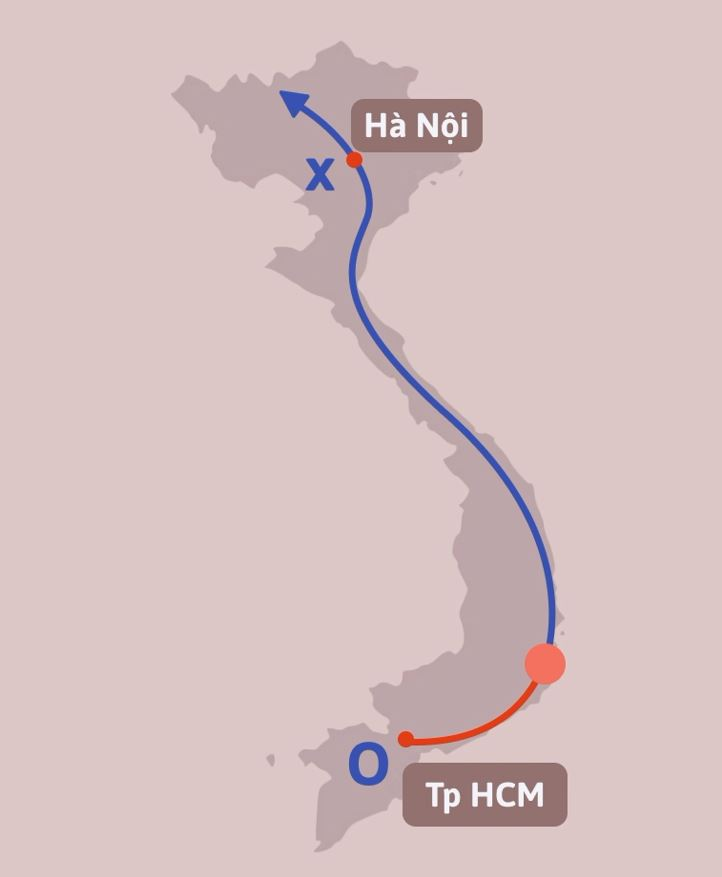
\includegraphics[scale=0.3]{figs/G10Y25B3-1}
%	\end{center}
%	\paragraph{Hệ tọa độ}
%	Muốn xác định vị trí của một điểm trên một mặt phẳng ta cần có hệ tọa độ với hai trục $Ox$ và $Oy$ vuông góc nhau, hình chiếu vuông góc của điểm xuống hai trục tọa độ đó chính là tọa độ của điểm đó.
%	\begin{center}
%		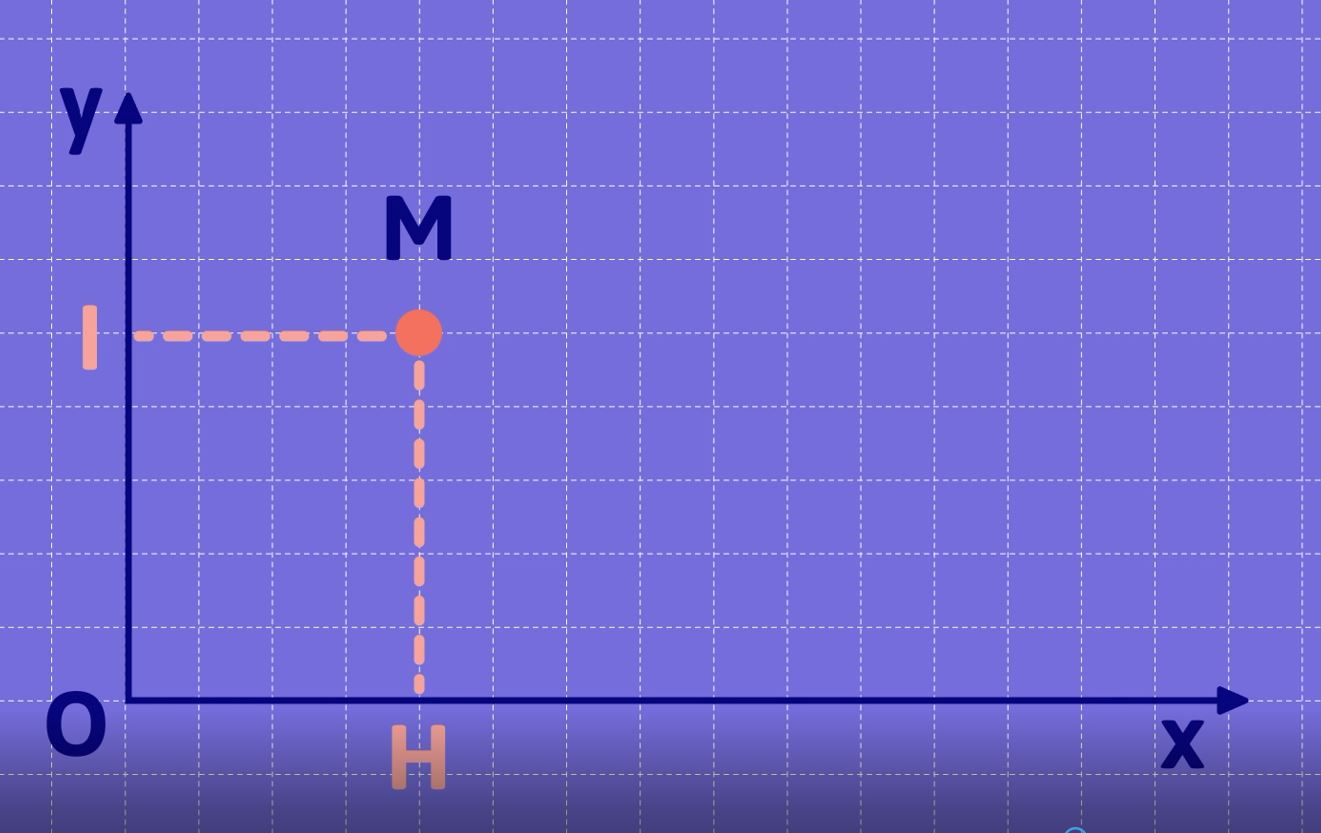
\includegraphics[scale=0.4]{figs/G10Y25B3-2}
%	\end{center}
%	\subsubsection{Cách xác định thời gian trong chuyển động}
%	\subsubsection{Mốc thời gian và đồng hồ}
%	Để mô tả chuyển động của một vật ta phải biết tọa độ của vật đó ở những thời điểm khác nhau. Muốn thế, ta phải chỉ rõ mốc thời gian và đo khoảng thời gian trôi đi kể từ mốc thời gian bằng một đồng hồ.
%	\subsubsection{Thời điểm và thời gian}
%	Nếu lấy mốc thời gian là thời điểm vật bắt đầu chuyển động (thời điểm 0) thì số chỉ của thời điểm sẽ trùng với số đo khoảng thời gian đã trôi qua kể từ mốc thời gian.
%	\subsection{Hệ quy chiếu}
%	Một hệ quy chiếu gồm:
%	\begin{itemize}
%		\item mốc tọa độ và một hệ tọa độ để đo vị trí;
%		\item mốc thời gian và một đồng hồ để xác định thời điểm.
%	\end{itemize}
	\subsubsection{Độ dịch chuyển và quãng đường đi được}
	\paragraph{Độ dịch chuyển}
	\begin{dn}
		Độ dịch chuyển được xác định bằng độ biến thiên toạ độ của vật
		$$d=x_2-x_1=\Delta x$$
	\end{dn}
	\begin{center}
		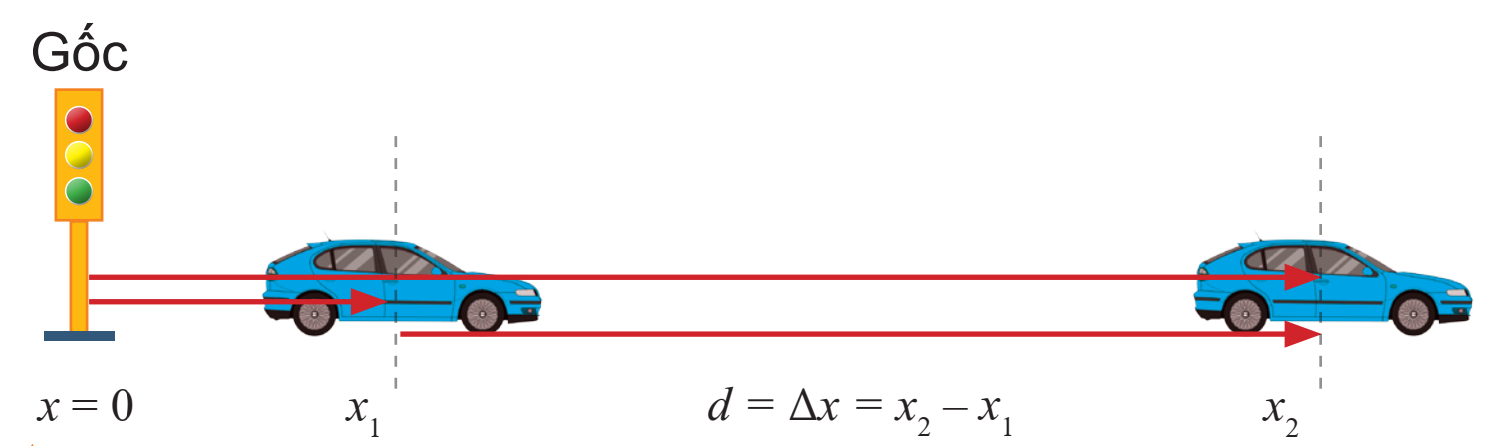
\includegraphics[scale=0.5]{figs/G10Y25B3-3}
		\captionof{figure}{Ví dụ thực tế về độ dịch chuyển của vật trên đường thẳng}
	\end{center}
	\begin{tc}
		Độ dịch chuyển có các đặc điểm sau:
		\begin{itemize}
			\item độ dịch chuyển là một đại lượng vector $\left(\vec{d}\right)$ có gốc tại vị trí ban đầu, hướng từ vị trí đầu đến vị trí cuối, độ lớn bằng khoảng cách giữa vị trí đầu và vị trí cuối.
			\item độ dịch chuyển là một đại lượng có thể nhận giá trị dương, âm hoặc bằng không. 
		\end{itemize}
	\end{tc}
	\paragraph{So sánh độ dịch chuyển và quãng đường đi được}
	\begin{longtable}{|m{20em}|m{20em}|}
		\hline
		\thead{Độ dịch chuyển $\left(\vec{d}\right)$} & \thead{Quãng đường $\left(s\right)$}\\
		\hline
		Là đại lượng vector. & Là đại lượng vô hướng.\\
		\hline
		Cho biết sự thay đổi vị trí của một vật (về hướng và độ dời). & Cho biết độ dài mà vật đi được.\\
		\hline
		Có thể nhận giá trị dương, âm hoặc bằng 0. & Có giá trị không âm.\\
		\hline
	\end{longtable}
	\begin{luuy}
		Khi vật chuyển động theo một hướng (chuyển động thẳng và không đổi chiều) thì độ lớn của độ dịch chuyển và quãng đường đi được bằng nhau $(d=s)$.
	\end{luuy}
	\subsubsection{Tốc độ trung bình - Vận tốc trung bình}
	\paragraph{Tốc độ trung bình}
	\begin{dn}
		Tốc độ trung bình $\overline{v}_{\text{tb}}$ là đại lượng đặc trưng cho mức độ nhanh hay chậm của chuyển động; được đo bằng thương số giữa quãng đường đi được $s$ và khoảng thời gian $t$ để đi hết quãng đường đó:
		\begin{equation}
			\overline{v}_{\text{tb}}=\dfrac{s}{t}.
		\end{equation}
	\end{dn}
	Trong hệ SI, đơn vị của tốc độ trung bình là \si{\meter/\second}. Các đơn vị khác cũng thường được sử dụng là \si{\kilo\meter/\hour}, \si{\centi\meter/\second}, \dots
	\begin{noidung}{Tốc độ tức thời}
		Tốc độ trung bình tính trong khoảng thời gian rất nhỏ là tốc độ tức thời (kí hiệu $v$) diễn tả sự nhanh, chậm của chuyển động tại thời điểm đó.
	\end{noidung}
	\begin{luuy}
		\begin{itemize}
			\item Khi một vật chuyển động với tốc độ tức thời không đổi, ta nói chuyển động của vật là chuyển động đều. Ngược lại, ta nói chuyển động của vật là không đều.
			\item Trên thực tế, tốc độ tức thời được hiển thị bởi tốc kế trên nhiều phương tiện giao thông.
		\end{itemize}
	\end{luuy}
	\paragraph{Vận tốc trung bình}
	\begin{dn}
		Vận tốc trung bình là đại lượng vectơ được xác định bằng thương số giữa độ dịch chuyển của vật và thời gian để vật thực hiện độ dịch chuyển đó
		$$v_\text{tb}=\dfrac{\vec{d}}{\Delta t}=\dfrac{\Delta \vec{x}}{\Delta t}.$$
	\end{dn}
	\begin{luuy}
		Tốc độ trung bình chỉ bằng độ lớn của vận tốc trung bình khi vật chuyển động thẳng không đổi chiều.
	\end{luuy}
	\subsubsection{Phương trình chuyển động thẳng đều}
	Xét một chất điểm chuyển động thẳng đều trên đường thẳng O$x$ với tốc độ $v$. Ở thời điểm ban đầu ($t_0=0$), vật ở vị trí A cách gốc O một đoạn $x_0$. Vào thời điểm $t$, vật ở vị trí M cách gốc O một đoạn $x$.  
	\begin{center}
		\begin{tikzpicture}
			\coordinate (O) at (0,0);
			\coordinate (A) at (2,0);
			\coordinate (M) at (5,0);
			\coordinate (x) at (8,0);
			\coordinate (O1) at ($(O)-(0,1cm)$);
			\coordinate (A1) at ($(A)-(0,1cm)$);
			\draw[->,thick] (O) -- (x);
			\foreach \i in {O,A}{
				\filldraw[black] (\i) circle (0.5mm);
			}
			\node[label=90:O] at (O){};	
			\node[label=90:A] at (A){};
			\node[label=90:M] at (M){};	
			\node[label=90:x] at (x){};	
			\draw[<->] (O1) -- (A1);
			\node [fill=white] (F1) at ($(O1)!0.5!(A1)$) {$x_0$};
			\coordinate (M1) at ($(M)-(0,1cm)$);
			\draw[<->] (A1) -- (M1);
			\node [fill=white] (F2) at ($(A1)!0.5!(M1)$) {$s$};
			\coordinate (O2) at ($(O)-(0,1.5cm)$);
			\coordinate (M2) at ($(M)-(0,1.5cm)$);
			\draw[<->] (O2) -- (M2);
			\node [fill=white] (F3) at ($(O2)!0.5!(M2)$) {$x$};
			\draw[dashed] (O) -- (O2);
			\draw[dashed] (A) -- (A1);
			\draw[dashed] (M) -- (M2);
			\filldraw[blue] (M) circle (0.5mm);
			%		\node[above of=O]()
		\end{tikzpicture}
	\end{center}
	
	Tọa độ của chất điểm sau thời gian chuyển động $t$ là:
	\begin{equation}
		x=x_0+s=x_0+vt.
	\end{equation}
	Phương trình dùng để xác định tọa độ của M theo thời gian được gọi là phương trình chuyển động của chất điểm M. Trong trường hợp này, M chuyển động thẳng đều nên phương trình này gọi là phương trình chuyển động thẳng đều của điểm M. 
	\subsubsection{Đồ thị độ dịch chuyển - Thời gian}
	\paragraph{Đồ thị độ dịch chuyển - thời gian}
	Đồ thị độ dịch chuyển - thời gian của hai vật A và B được mô tả như hình \ref{fig:5.1}
	\begin{center}
		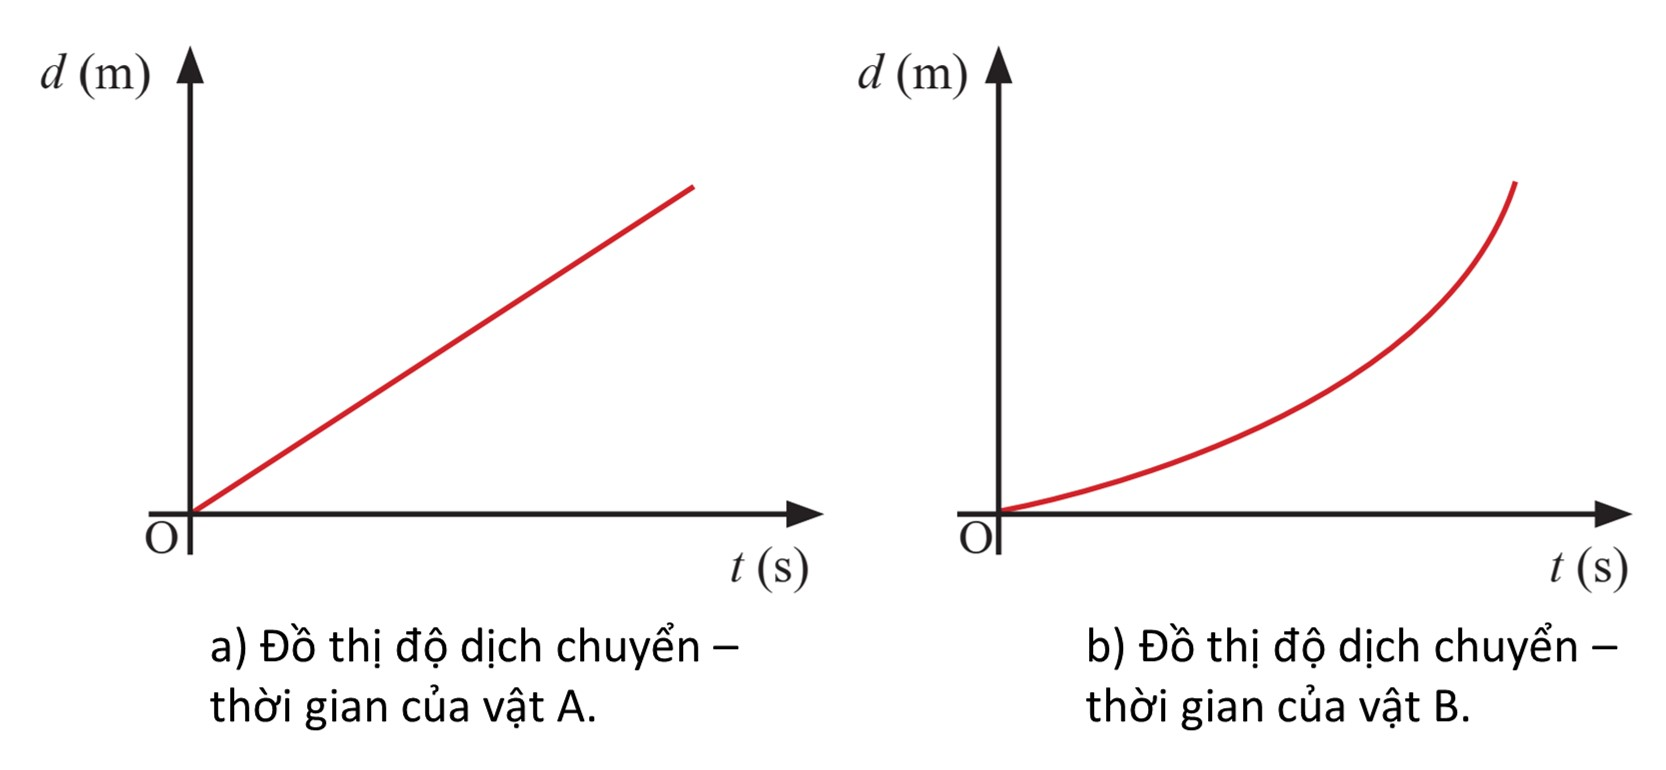
\includegraphics[scale=0.5]{figs/G10Y25B3-18}
		\captionof{figure}{}
		\label{fig:5.1}
	\end{center}
	Từ các đồ thị $\left(d-t\right)$, ta có nhận xét:
	\begin{enumerate}[label=\alph*)]
		\item Đồ thị $\left(d-t\right)$ mô tả chuyển động của vật $A$ là đường thẳng đi qua gốc toạ độ. Chuyển động của vật $A$ là chuyển động thẳng đều.
		\item Đồ thị $\left(d-t\right)$ mô tả chuyển động của vật $B$ là đường cong qua gốc toạ độ. Độ dịch chuyển của vật B trong những khoảng thời gian bằng nhau tăng lên nên chuyển động của vật B là chuyển động thẳng nhanh dần.
	\end{enumerate}
	\paragraph{Xác định vận tốc từ độ dốc của đồ thị độ dịch chuyển - thời gian}
	\begin{tc}
		Vận tốc tức thời của vật tại một thời điểm được xác định bởi độ dốc của tiếp tuyến với đồ thị $\left(d-t\right)$ tại thời điểm đang xét.\\
		Tốc độ tức thời tại một thời điểm chính là độ lớn của độ dốc tiếp tuyến của đồ thị $\left(d-t\right)$ tại điểm đó.
	\end{tc}
	\begin{center}
		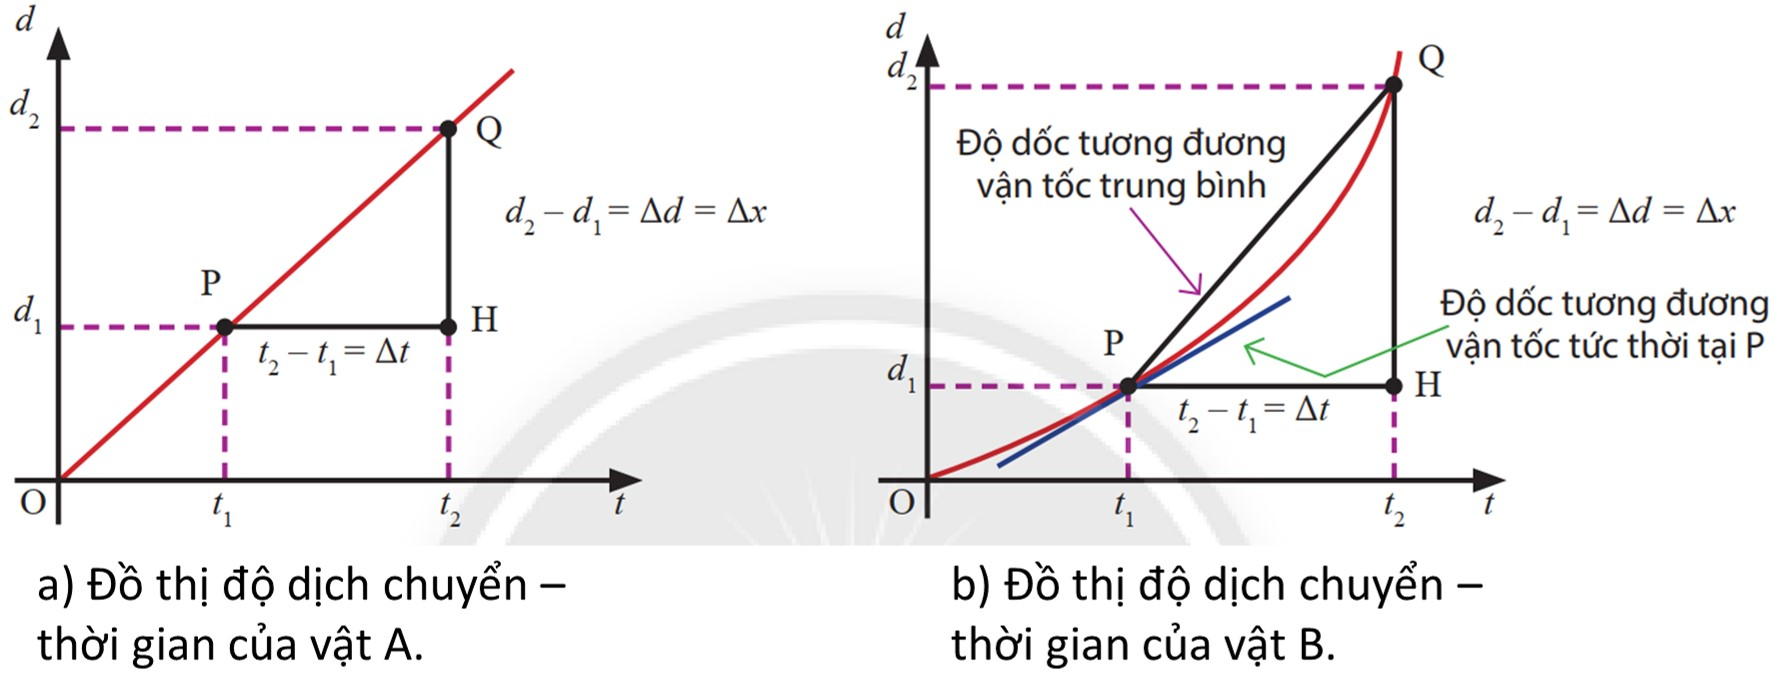
\includegraphics[scale=0.5]{figs/G10Y25B3-19}
		\captionof{figure}{}
		\label{fig:5.2}
	\end{center}
	
\end{tomtat}
\subsection{VÍ DỤ MINH HỌA}
\begin{dang}{Thực hiện xác định thời điểm và thời gian (mốc thời gian và đồng hồ)}
\end{dang}
\begin{vd}
	Giờ Berlin chậm hơn giờ Hà Nội 5 giờ. Trận bóng đá diễn ra tại Beclin lúc 19h00 ngày 2-9-2021. Khi đó theo giờ Hà Nội là
	\choice
	{14h00 ngày 3-9-2021}
	{\True 0h00 ngày 3-9-2021}
	{0h00 ngày 2-9-2021}
	{14h00 ngày 2-9-2021}
	\loigiai{	
		Giờ Berlin chậm hơn giờ Hà Nội 5 giờ, nghĩa là
		$$t_{\text{B}}+\SI{5}{\hour}=t_{\text{HN}}.$$
		Trận bóng đá diễn ra tại Berlin lúc 19h00 ngày 2-9-2021. Thời điểm đó theo giờ Hà Nội là:
		$$t_{\text{HN}}=t_{\text{B}}+\SI{5}{\hour}=19\text{h}00 + 5\text{h} = 24\text{h}00$$
		Một ngày chỉ có 24 giờ nên thời điểm trên đã bước sang ngày hôm sau. Do đó, trận bóng trên diễn ra vào lúc 0h00 ngày 3-9-2021 giờ Hà Nội. 	
	}
\end{vd}

\begin{vd}
	Theo lịch trình tại bến xe ở Hà Nội thì ô tô chở khách trên tuyến Hà Nội - Hải Phòng chạy từ Hà Nội lúc 6 giờ sáng, đi qua Hải Dương lúc 7 giờ 15 phút sáng và tới Hải Phòng lúc 8 giờ 50 phút sáng cùng ngày. Hà Nội cách Hải Dương 60 km và cách Hải Phòng $\SI{105}{km}$. Xe ô tô chạy liên tục không nghỉ dọc đường, chỉ dừng lại 10 phút tại bến xe Hải Dương để đón, trả khách. Tính khoảng thời gian chuyển động và quãng đường đi được của các hành khách sau:
	\begin{enumerate}[label=\alph*)]
		\item Hành khách lên xe tại Hà Nội đi Hải Phòng.
		\item Hành khách lên xe tại Hải Dương đi Hải Phòng.
	\end{enumerate}
	\loigiai{
		\begin{enumerate}[label=\alph*)]
			\item Đối với hành khách lên xe tại Hà Nội đi Hải Phòng, chọn bến xe Hà Nội làm mốc và thời điểm ô tô bắt đầu xuất phát là mốc thời gian.
			
			Khoảng thời gian chuyển động là:	
			\begin{center}
				(8 giờ 50 phút - 6 giờ) - 10 phút = 2 giờ 40 phút.
			\end{center}
			Quãng đường đi được đúng bằng độ dài của đoạn đường Hà Nội - Hải Phòng là $\SI{105}{km}$.
			\item Đối với hành khách lên xe tại Hải Dương đi Hải Phòng, chọn bến xe Hải Dương làm mốc và thời điểm ô tô bắt đầu xuất phát là mốc thời gian.
			
			Khoảng thời gian chuyển động là:
			\begin{center}
				8 giờ 50 phút - (7 giờ 15 phút + 10 phút) = 1 giờ 25 phút.
			\end{center}
			Quãng đường đi được là:
			$$\SI{105}{km}-\SI{60}{km}=\SI{45}{km}.$$
		\end{enumerate}
	}
\end{vd}

\begin{dang}{So sánh được quãng đường đi được và độ dịch chuyển.}
	\begin{center}
		\begin{tabular}{|M{8cm}|M{8cm}|}
			\hline
			\thead{Độ dịch chuyển $\left(\vec{d}\right)$} & \thead{Quãng đường $\left(s\right)$}\\
			\hline
			Đại lượng vector \textit{(gốc tại vị trí ban đầu, hướng từ vị trí đầu đến vị trí cuối)}. & Đại lượng vô hướng.\\
			\hline
			Xác định bằng độ biến thiên tọa độ: $d=x_2-x_1=\Delta x$. & Xác định bằng tổng chiều dài đoạn đường đi.\\
			\hline
			Có thể nhận giá trị dương, âm hoặc bằng 0. & Nhận giá trị không âm.\\
			\hline
			
		\end{tabular}
	\end{center}
\end{dang}
\begin{vd}
	Xét quãng đường $AB$ dài $\SI{1000}{\meter}$ với $A$ là vị trí nhà của em và $B$ là vị trí của bưu điện. Tiệm tạp hóa nằm tại vị trí $C$ là trung điểm của $AB$. Nếu chọn nhà em làm gốc tọa độ và chiều dương hướng từ nhà em đến bưu điện. Hãy xác định độ dịch chuyển và quãng đường đi được của em trong các trường hợp:
	\begin{center}
		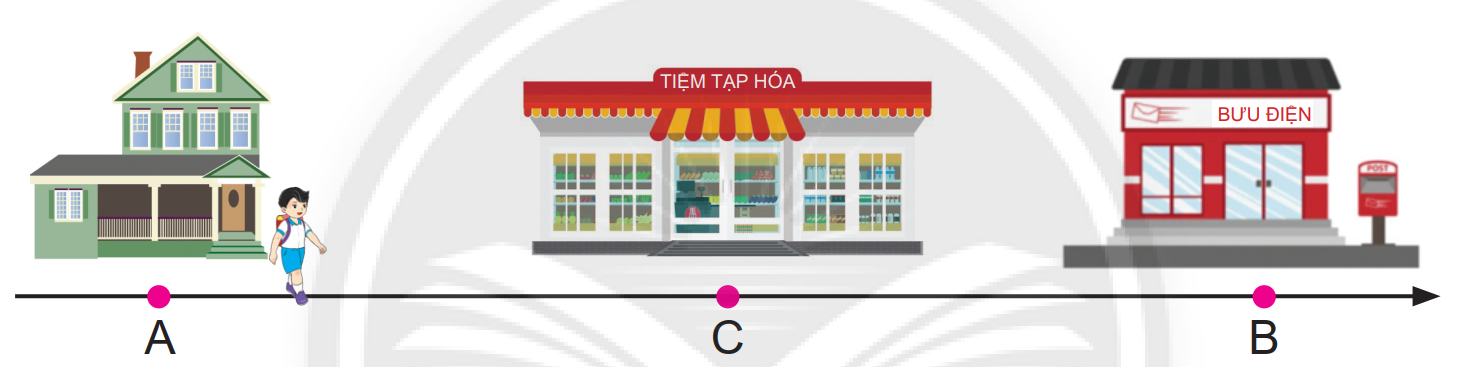
\includegraphics[width=0.6\linewidth]{figs/G10Y25B3-4}
	\end{center}
	\begin{enumerate}[label=\alph*)]
		\item Đi từ nhà đến bưu điện.
		\item Đi từ nhà đến bưu điện rồi quay lại tiệm tạp hóa.
		\item Đi từ nhà đến tiệm tạp hóa rồi quay về. 
	\end{enumerate}	
	\loigiai{
		\begin{enumerate}[label=\alph*)]
			\item Độ dịch chuyển $d=AB=x_B-x_A=\SI{1000}{\meter}-\SI{0}{\meter}=\SI{1000}{\meter}$.\\
			Quãng đường đi được $s=AB=\SI{1000}{\meter}$.
			\item Độ dịch chuyển $d=AC=x_A-x_C=\SI{500}{\meter}-\SI{0}{\meter}=\SI{500}{\meter}$.\\
			Quãng đường đi được $s=AB+BC=\SI{1500}{\meter}$.
			\item Độ dịch chuyển $d=x_A-x_A=\SI{0}{\meter}$.\\
			Quãng đường đi được $s=2AC=\SI{1000}{\meter}$.
		\end{enumerate}
	}
\end{vd}

\begin{vd}
	Một vận động viên chạy từ cổng Dinh Thống Nhất (A) đến Thảo Cầm Viên (D) theo hai quỹ đạo khác nhau. Hãy xác định độ dịch chuyển và quãng đường chạy được của người vận động viên trong 2 trường hợp trên.
	\begin{center}
		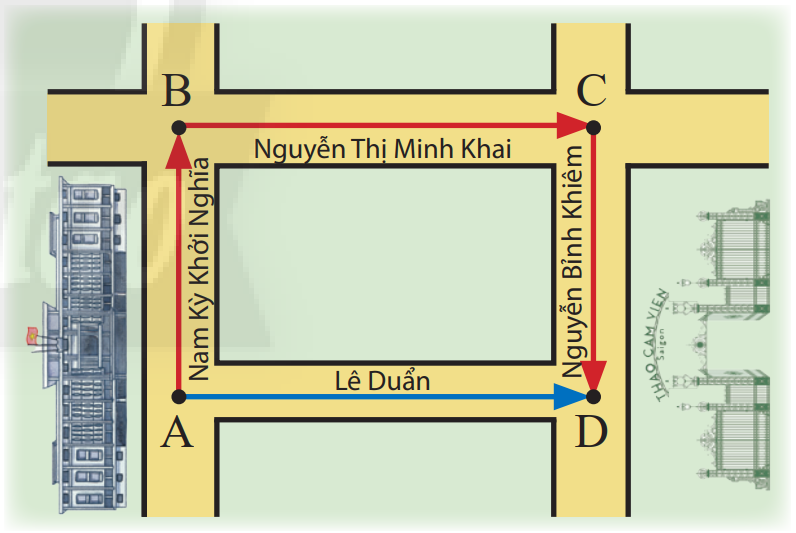
\includegraphics[width=0.5\linewidth]{figs/G10Y25B3-5}
	\end{center}
	\loigiai{
		\textbf{Trường hợp 1:} Nếu vận động viên chạy theo đường Lê Duẩn thì\\
		Độ dời $\vec{d}=\overrightarrow{AD}$, về độ lớn thì $d=AD$.\\
		Quãng đường $s=AD$.\\
		\textbf{Trường hợp 2:} Nếu vận động viên chạy theo đường Nam Kì Khởi Nghĩa qua đường Nguyễn Thị Minh Khai rồi mới đến Thảo Cầm Viên ở đường Nguyễn Bỉnh Khiêm thì\\
		Độ dời $\vec{d}=\overrightarrow{AD}$, về độ lớn thì $d=AD$.\\
		Quãng đường $s=AB+BC+CD$.
	}
\end{vd}
\begin{dang}{Mối liên hệ giữa quãng đường đi và tốc độ trung bình}
$$\overline{v}_{\mathrm{tb}}=\dfrac{s}{t}.$$
\end{dang}
\begin{vd}
	Một ô tô đi trên con đường bằng phẳng với tốc độ trung bình $v = \SI{60}{km/h}$, trong thời gian 5 phút, sau đó lên dốc 3 phút với tốc độ trung bình $v = \SI{40}{km/h}$. Tính quãng đường ô tô đã đi trong cả giai đoạn.
	\loigiai{
		Quãng đường ô tô đi được trên đoạn đường phẳng
		$$s_1 =v_1t_1 =\SI{60}{\kilo\meter/\hour}\cdot\SI{5}{\minute}=\dfrac{\SI{60}{\kilo\meter}}{\SI{1}{\hour}}\cdot\SI{5}{\minute}=\dfrac{\SI{60}{\kilo\meter}}{\SI{60}{\minute}}\cdot\SI{5}{\minute}=\SI{5}{km}.$$
		
		Quãng đường ô tô lên dốc
		$$s_2 = v_2t_2=\SI{40}{\kilo\meter/\hour}\cdot\SI{3}{\minute}=\dfrac{\SI{40}{\kilo\meter}}{\SI{1}{\hour}}\cdot\SI{3}{\minute}=\dfrac{\SI{40}{\kilo\meter}}{\SI{60}{\minute}}\cdot\SI{3}{\minute} = \SI{2}{km}.$$
		
		Quãng đường ô tô đã đi trong cả giai đoạn
		$$s = s_1+s_2 = \SI{7}{km}.$$
	}
\end{vd}

\begin{vd}
	Hai xe cùng chuyển động đều trên đường thẳng. Nếu chúng đi ngược chiều thì cứ 30 phút khoảng cách của chúng giảm $\SI{40}{km}$. Nếu chúng đi cùng chiều thì cứ sau 20 phút khoảng cách giữa chúng giảm $\SI{8}{km}$. Tính tốc độ của mỗi xe.
	\loigiai{
		Nếu đi ngược chiều thì 
		\begin{eqnarray}
			s_1+s_2 &=&(v_1+v_2)t_1 =\SI{40}{\kilo\meter}\nonumber\\
			\Rightarrow\qquad v_1+v_2&=&\dfrac{\SI{40}{\kilo\meter}}{\SI{0.5}{\hour}}=\SI{80}{\kilo\meter/\hour}\label{eq:tongv}
		\end{eqnarray}
		Nếu đi cùng chiều thì	
		\begin{eqnarray}
			s'_1-s'_2 &=&(v_1-v_2)t_2 =\SI{8}{\kilo\meter}\nonumber\\
			\Rightarrow\qquad v_1-v_2&=&\dfrac{\SI{8}{\kilo\meter}}{\xsi{\dfrac{1}{3}}{\hour}}=\SI{24}{\kilo\meter/\hour}\label{eq:hieuv}
		\end{eqnarray}
		
		Giải hệ gồm 2 phương trình \eqref{eq:tongv} và \eqref{eq:hieuv}, ta tìm được:
		$$v_1 = \SI{52}{km/h};\quad v_2 =\SI{28}{km/h}.$$
	}
\end{vd}
\begin{dang}{Xác định tốc độ trung bình của chuyển động thẳng khi biết tốc độ trung bình trên từng giai đoạn}
\end{dang}
\begin{vd}
	Một xe chạy trong $\SI{5}{\hour}$, $\SI{2}{\hour}$ đầu xe chạy với tốc độ trung bình $\SI{60}{\kilo\meter/\hour}$, $\SI{3}{\hour}$ sau xe chạy với tốc độ trung bình $\SI{40}{\kilo\meter/\hour}$. Tính tốc độ trung bình của xe trong suốt thời gian chuyển động.
	\loigiai{
		Quãng đường xe đi được trong $\SI{2}{\hour}$ đầu 
		\begin{equation*}
			s_1 = v_1t_1 =\SI{60}{\kilo\meter/\hour}\cdot\SI{2}{\hour} = \SI{120}{\kilo\meter}.
		\end{equation*}
		
		Quãng đường xe đi được trong $\SI{3}{\hour}$ sau 
		\begin{equation*}
			s_2 = v_2t_2 =\SI{40}{\kilo\meter/\hour}\cdot\SI{3}{\hour}= \SI{120}{\kilo\meter}.
		\end{equation*}
		
		Tốc độ trung bình của xe trong suốt thời gian chuyển động 
		\begin{equation*}
			v_{\text{tb}}=\dfrac{s}{t}=\dfrac{s_1+s_2}{t_1+t_2}=\dfrac{\SI{120}{\kilo\meter}+\SI{120}{\kilo\meter}}{\SI{2}{\hour}+\SI{3}{\hour}}=\dfrac{\SI{240}{\kilo\meter}}{\SI{5}{\hour}}=\SI{48}{\kilo\meter/\hour}.
		\end{equation*}
	}
\end{vd}

\begin{vd}
	Một ô tô đi từ A đến B. Đầu chặng ô tô đi 1/4 tổng thời gian với tốc độ $v_1=\SI{50}{\kilo\meter/\hour}$. Giữa chặng ô tô đi 1/2 tổng thời gian với tốc độ $v_2=\SI{40}{\kilo\meter/\hour}$. Cuối chặng ô tô đi 1/4 tổng thời gian với tốc độ $v_3=\SI{20}{\kilo\meter/\hour}$. Tính tốc độ trung bình của ô tô?
	\loigiai{
		Quãng đường ô tô đi đầu chặng 
		\begin{equation*}
			s_1=v_1t_1=v_1\cdot\dfrac{t}{4}.
		\end{equation*}
		
		Quãng đường ô tô đi giữa chặng 
		\begin{equation*}
			s_2=v_2t_2=v_2\cdot\dfrac{t}{2}.
		\end{equation*}
		
		Quãng đường ô tô đi cuối chặng 
		\begin{equation*}
			s_3=v_3t_3=v_3\cdot\dfrac{t}{4}.
		\end{equation*}
		
		Tốc độ trung bình của ô tô trên cả hành trình 
		\begin{equation*}
			v_{\text{tb}}=\dfrac{s_1+s_2+s_3}{t}=\dfrac{v_1\cdot\dfrac{t}{4}+v_2\cdot\dfrac{t}{2}+v_3\cdot\dfrac{t}{4}}{t}=\dfrac{v_1}{4}+\dfrac{v_2}{2}+\dfrac{v_3}{4}=\SI{37,5}{\kilo\meter/\hour}.
		\end{equation*}
	}
\end{vd}
\begin{dang}{Nhận biết được phương trình chuyển động thẳng đều}
	Phương trình tọa độ của vật chuyển động thẳng đều:
	$$x=x_0+vt.$$
\end{dang}
\begin{vd}
	Trong các phương trình chuyển động thẳng đều sau đây, phương trình nào biểu diễn chuyển động không xuất phát từ gốc tọa độ và ban đầu hướng về gốc tọa độ:
	\choice
	{\True $x = 80 - 30t$}
	{$x = 15 + 40t$}
	{$x = -6t$}
	{$x = -10 - 6t$}
	\loigiai{
		Phương trình chuyển động của vật là 
		$$x=x_0 +vt.$$	
		Chuyển động không xuất phát từ gốc tọa độ thì $x_0 \neq 0$.
		
		Ban đầu vật hướng về gốc tọa độ thì vị trí ban đầu và vận tốc của vật phải thỏa mãn 
		\begin{equation*}
			\left\lbrace
			\begin{array}{rl}
				x_0&<0,\\
				v&>0
			\end{array}
			\right.
			\qquad\text{hoặc}\qquad
			\left\lbrace
			\begin{array}{rl}
				x_0&>0,\\
				v&<0
			\end{array}
			\right.
		\end{equation*}
		Hình vẽ sau minh họa hai trường hợp này.
		\begin{center}
			\begin{tikzpicture}
				\coordinate (O) at (0,0);
				\coordinate (A) at (-3,0);
				\coordinate (A1) at ($(A)+(1,0)$);
				\coordinate (M) at (4,0);
				\coordinate (M1) at ($(M)-(1,0)$);
				\coordinate (x) at (6,0);
				\coordinate (X) at (-4,0);
				\draw[->] (X) -- (x);
				\foreach \i in {O,A,M}{
					\filldraw[black] (\i) circle (0.5mm);
				}
				\draw[->,very thick,blue] (A) -- (A1);
				\draw[->,very thick,red] (M) -- (M1);
				\node[label=90:O] at (O){};	
				\node[label=90:$\vec{v}$]at (A1){};
				\node[label=90:$\vec{v}$]at (M1){};
				\node[align=center,below=0.2cm of A](Mnode){$x_0<0$\\$v>0$};
				\node[align=center,below=0.2cm of M](Mnode){$x_0>0$\\$v<0$};
				\node[label=90:$x$]at (x){};
			\end{tikzpicture}
		\end{center}
		Trong các lựa chọn, chỉ có lựa chọn A ($x = 80 - 30t$) thỏa mãn với điều kiện trên.
	}
\end{vd}
\begin{dang}{Xây dựng phương trình, xác định các đại lượng trong phương trình chuyển động thẳng đều.}
\end{dang}
\begin{vd}
	Một vật chuyển động thẳng đều với tốc độ $\SI{2}{m/s}$. Lúc $t = \SI{2}{s}$ vật có tọa độ $\SI{5}{m}$. Phương trình chuyển động của vật là 
	\choice
	{\True $x=2t+1\qquad\left(\si{\meter}, \si{\second}\right)$.}
	{$x=-2t +5\qquad\left(\si{\meter}, \si{\second}\right)$.}
	{$x=2t+5\qquad\left(\si{\meter}, \si{\second}\right)$.}
	{$x=-2t+1\qquad\left(\si{\meter}, \si{\second}\right)$.}
	\loigiai{
		Phương trình tọa độ của vật có dạng: 
		$$x=x_0 +vt.$$
		
		Thay $x=\SI{5}{m}$, $v=\SI{2}{m/s}$, $t=\SI{2}{s}$ vào ta suy ra 
		\begin{align*}
			x_0=x-vt=\SI{5}{m}-\SI{2}{\meter/\second}\cdot\SI{2}{s}=\SI{1}{m}.
		\end{align*}
		
		Vậy phương trình chuyển động của vật là:
		
		$$x=1+2t =2t+1\qquad\left(\si{\meter}, \si{\second}\right).$$
	}
\end{vd}

\begin{vd}
	Trên đường thẳng từ nhà đến chỗ làm việc của A, cùng một lúc xe 1 khởi hành từ nhà đến chỗ làm với $v_1=\SI{80}{\kilo\meter/\hour}$. Xe 2 từ chỗ làm đi cùng chiều xe 1 với $v_2=\SI{60}{\kilo\meter/\hour}$. Biết quãng đường từ nhà đến chỗ làm là $\SI{40}{\kilo\meter}$. Lập phương trình chuyển động của mỗi xe với cùng hệ quy chiếu.
	\loigiai{
		Chọn hệ quy chiếu gồm:
		\begin{itemize}
			\item Chiều dương cùng chiều với chiều chuyển động của hai xe;
			\item Gốc tọa độ tại nhà (vị trí ban đầu của xe 1);
			\item Mốc thời gian lúc hai xe bắt đầu xuất phát.
		\end{itemize}
		
		Xe 1 có phương trình chuyển động:
		\begin{equation*}
			x_1=x_0 + v_1t = 80t\qquad\left(\si{\kilo\meter}, \si{\hour}\right).
		\end{equation*}
		Xe 2 có phương trình chuyển động:
		\begin{equation*}
			x_2=x_0 + v_2t =  40+60t\qquad\left(\si{\kilo\meter}, \si{\hour}\right).
		\end{equation*}
	}
\end{vd}

\begin{vd}
	Hai vật chuyển động ngược chiều qua A và B cùng một lúc. Vật qua A có tốc độ $v_1=\SI{10}{\meter/\second}$, vật qua B có tốc độ $v_2=\SI{15}{\meter/\second}$. Cho biết AB có chiều dài $\SI{100}{m}$. Lấy trục tọa độ là đường thẳng AB, gốc tọa độ ở B, chiều dương từ A sang B, mốc thời gian là lúc chúng cùng qua A và B. Lập phương trình chuyển động của mỗi vật.
	\loigiai{
		Hệ quy chiếu gồm:
		\begin{itemize}
			\item Gốc tọa độ tại B;
			\item Chiều dương từ A sang B;
			\item Mốc thời gian lúc hai vật cùng qua A và B.
		\end{itemize}
		
		Xác định các thông số cho từng vật:
		\begin{itemize}
			\item Vật qua A:
			\begin{itemize}
				\item Vị trí ban đầu ($x_{0\text{A}}$): Vì gốc tọa độ ở B và chiều dương từ A sang B, A cách B $\SI{100}{m}$ theo chiều âm (ngược chiều dương), nên $x_{0\text{A}} = -\SI{100}{m}$.
				\item Vận tốc ($v_{\text{A}}$): Vật chuyển động từ A theo chiều dương (tức là hướng từ A sang B), nên $v_{\text{A}} = +\SI{10}{m/s}$.
			\end{itemize}
			\item Vật qua B:
			\begin{itemize}
				\item Vị trí ban đầu ($x_{0\text{B}}$): Vật ở B, mà B là gốc tọa độ, nên $x_{0\text{B}} = \SI{0}{m}$.
				\item Vận tốc ($v_{\text{B}}$): Vật chuyển động ngược chiều qua A, tức là từ B hướng về A (ngược chiều dương), nên $v_{\text{B}} = -\SI{15}{m/s}$.
			\end{itemize}
		\end{itemize}
		
		Phương trình chuyển động của vật qua A là:
		\begin{equation*}
			x_\text{A}=x_{0\text{A}} + v_\text{A}t = -\SI{100}{m} + \SI{10}{m/\second} \cdot t = -100+10t\qquad\left(\si{\meter}, \si{\second}\right).
		\end{equation*}
		
		Phương trình chuyển động của vật qua B là:
		\begin{equation*}
			x_\text{B}=x_{0\text{B}} + v_\text{B}t = \SI{0}{m} + \left(-\SI{15}{m/\second}\right) \cdot t = -15t\qquad\left(\si{\meter}, \si{\second}\right).
		\end{equation*}
	}
\end{vd}
\begin{dang}{Xác định vị trí, thời điểm hai vật chuyển động thẳng đều gặp nhau}
\end{dang}
\begin{vd}
	Hai vật chuyển động ngược chiều qua A và B cùng một lúc. Vật qua A có tốc độ $v_1=\SI{10}{m/s}$, vật qua B có tốc độ $v_2=\SI{15}{m/s}$. Cho biết AB có chiều dài $\SI{100}{m}$. Xác định vị trí và thời điểm chúng gặp nhau.
	\loigiai{
		Chọn gốc tọa độ ở vị trí A, gốc thời gian ở thời điểm hai vật bắt đầu chuyển động (lúc chúng ở A và B). Chiều dương trục toạ độ hướng từ A sang B.
		
		Phương trình chuyển động của vật qua A:
		\begin{itemize}
			\item Vị trí ban đầu $x_{01} = \SI{0}{m}$.
			\item Vận tốc $v_1 = \SI{10}{m/s}$.
			\item Phương trình: $x_1 = 10t\qquad\left(\si{\meter}, \si{\second}\right).$
		\end{itemize}
		
		Phương trình chuyển động của vật qua B:
		\begin{itemize}
			\item Vị trí ban đầu $x_{02} = \SI{100}{m}$.
			\item Vận tốc $v_2 = -\SI{15}{m/s}$ (vì chuyển động ngược chiều dương, tức là hướng về A).
			\item Phương trình: $x_2 = 100-15t\qquad\left(\si{\meter}, \si{\second}\right).$
		\end{itemize}
		
		Hai vật gặp nhau khi chúng có cùng tọa độ:
		$$x_1 = x_2$$
		$$\Rightarrow 10t = 100 - 15t$$
		$$25t = 100$$
		$$t = \dfrac{100}{25} = \SI{4}{s}.$$
		
		Thời điểm hai vật gặp nhau là $\SI{4}{s}$ sau khi bắt đầu chuyển động.
		
		Vị trí hai vật gặp nhau (thay $t = \SI{4}{s}$ vào một trong hai phương trình):
		$$x_1 = 10 \cdot 4 = \SI{40}{m}.$$
		Hoặc $$x_2 = 100 - 15 \cdot 4 = 100 - 60 = \SI{40}{m}.$$
		
		Vậy hai vật gặp nhau tại vị trí cách A một khoảng $\SI{40}{m}$ vào thời điểm $\SI{4}{s}$.
	}
\end{vd}

\begin{vd}
	Lúc 7 giờ, một người ở A chuyển động thẳng đều với tốc độ $v_A = \SI{36}{\kilo\meter/\hour}$ đuổi theo người ở B đang chuyển động với tốc độ $v_B = \SI{5}{m/s}$. Biết $AB = \SI{18}{\kilo\meter}$. Hai người đuổi kịp nhau tại nơi cách A một khoảng:
	\choice
	{$\SI{58}{\kilo\meter}$}
	{$\SI{46}{\kilo\meter}$}
	{\True $\SI{36}{\kilo\meter}$}
	{$\SI{24}{\kilo\meter}$}
	\loigiai{
		Đổi đơn vị tốc độ của người ở B:
		$$v_B = \SI{5}{m/s} = 5 \cdot \dfrac{3600}{1000}\ \si{\kilo\meter/\hour} = \SI{18}{\kilo\meter/\hour}.$$
		
		Chọn hệ quy chiếu:
		\begin{itemize}
			\item Gốc tọa độ tại A.
			\item Chiều dương trục tọa độ hướng từ A đến B.
			\item Gốc thời gian lúc 7 giờ.
		\end{itemize}
		
		Phương trình chuyển động của người ở A (người 1):
		\begin{itemize}
			\item Vị trí ban đầu $x_{0A} = \SI{0}{\kilo\meter}$.
			\item Vận tốc $v_A = +\SI{36}{\kilo\meter/\hour}$.
			\item Phương trình: $x_A = 36t\qquad\left(\si{\kilo\meter}, \si{\hour}\right).$
		\end{itemize}
		
		Phương trình chuyển động của người ở B (người 2):
		\begin{itemize}
			\item Vị trí ban đầu $x_{0B} = \SI{18}{\kilo\meter}$.
			\item Vận tốc $v_B = +\SI{18}{\kilo\meter/\hour}$.
			\item Phương trình: $x_B = 18+18t\qquad\left(\si{\kilo\meter}, \si{\hour}\right).$
		\end{itemize}
		
		Khi hai người gặp nhau, tọa độ của họ trùng nhau:
		$$x_A = x_B$$
		$$36t = 18 + 18t$$
		$$36t - 18t = 18$$
		$$18t = 18$$
		$$t = \SI{1}{\hour}.$$
		
		Thời điểm gặp nhau là $\SI{1}{\hour}$ sau 7 giờ, tức là lúc 8 giờ.
		
		Vị trí gặp nhau cách A một khoảng:
		$$x_A = 36t = \SI{36}{\kilo\meter/\hour} \cdot 1\ \si{\hour} = \SI{36}{\kilo\meter}.$$
		
		Vậy hai người đuổi kịp nhau tại nơi cách A một khoảng $\SI{36}{\kilo\meter}$.
	}
\end{vd}

\begin{vd}
	Xe thứ nhất đi từ A đến B mất 8 giờ, xe thứ hai đi từ B đến A mất 6 giờ. Nếu hai xe khởi hành cùng một lúc từ A và B để đến gần nhau thì sau 3 giờ hai xe cách nhau $\SI{30}{\kilo\meter}$. Tính chiều dài của quãng đường AB.
	\loigiai{
		Gọi $S$ là chiều dài quãng đường AB.
		Gọi $v_1$ và $v_2$ lần lượt là tốc độ của xe thứ nhất và xe thứ hai.
		Theo đề bài:
		Xe thứ nhất đi từ A đến B mất $\SI{8}{\hour}$, nên $v_1 = \dfrac{S}{\SI{8}{\hour}}$.
		Xe thứ hai đi từ B đến A mất $\SI{6}{\hour}$, nên $v_2 = \dfrac{S}{\SI{6}{\hour}}$.
		
		Chọn gốc tọa độ tại vị trí A, chiều dương từ A đến B và gốc thời gian là lúc 2 xe xuất phát.
		
		Phương trình chuyển động của xe thứ nhất (xuất phát từ A):
		$$x_1 = v_1 t = \left(\dfrac{S}{\SI{8}{\hour}}\right) \cdot t.$$
		
		Phương trình chuyển động của xe thứ hai (xuất phát từ B, chuyển động ngược chiều dương):
		$$x_2 = S - v_2 t = S - \left(\dfrac{S}{\SI{6}{\hour}}\right) \cdot t.$$
		
		Sau $\SI{3}{\hour}$ ($t = 3\ \si{\hour}$), hai xe cách nhau $\SI{30}{\kilo\meter}$. Điều này có nghĩa là giá trị tuyệt đối hiệu tọa độ của chúng bằng $\SI{30}{\kilo\meter}$:
		$$|x_1(3) - x_2(3)| = \SI{30}{\kilo\meter}.$$
		
		Thay $t = 3\ \si{\hour}$ vào các phương trình tọa độ:
		$$x_1(3) = \dfrac{S}{\SI{8}{\hour}} \cdot \SI{3}{\hour} = \dfrac{3S}{8}.$$
		$$x_2(3) = S - \dfrac{S}{\SI{6}{\hour}} \cdot \SI{3}{\hour} = S - \dfrac{3S}{6} = S - \dfrac{S}{2} = \dfrac{S}{2}.$$
		
		Vì hai xe đi đến gần nhau, chúng chưa gặp nhau và xe 2 sẽ ở phía trước xe 1 (do $S/2 > 3S/8$ khi $S>0$), nên $x_2 > x_1$.
		Vậy, $|x_1(3) - x_2(3)| = x_2(3) - x_1(3) = \SI{30}{\kilo\meter}.$
		$$\dfrac{S}{2} - \dfrac{3S}{8} = \SI{30}{\kilo\meter}$$
		$$\dfrac{4S - 3S}{8} = \SI{30}{\kilo\meter}$$
		$$\dfrac{S}{8} = \SI{30}{\kilo\meter}$$
		$$S = \SI{30}{\kilo\meter} \cdot 8 = \SI{240}{\kilo\meter}.$$
		
		Chiều dài của quãng đường AB là $\SI{240}{\kilo\meter}$.
	}
\end{vd}

\begin{vd}
	Hai vật chuyển động ngược chiều qua A và B cùng một lúc. Vật qua A có tốc độ $v_1=\SI{10}{\meter/\second}$, vật qua B có tốc độ $v_2=\SI{15}{\meter/\second}$. Cho biết AB có chiều dài $\SI{100}{m}$. Xác định vị trí và thời điểm chúng cách nhau $\SI{25}{\meter}$.
	\loigiai{
		Chọn gốc tọa độ ở A, chiều dương trục toạ độ hướng từ A đến B và gốc thời gian là thời điểm hai vật đang đi qua A và B. Gọi $S=\SI{100}{m}$ là chiều dài đoạn AB.
		
		Phương trình chuyển động của vật qua A:
		$$x_1=v_1t = 10t\qquad\left(\si{\meter}, \si{\second}\right).$$
		
		Phương trình chuyển động của vật qua B:
		$$x_2=S-v_2t = 100-15t\qquad\left(\si{\meter}, \si{\second}\right).$$
		
		Khi hai vật cách nhau $d=\SI{25}{m}$, ta có:
		$$d = |x_1 - x_2| = \SI{25}{m}.$$
		$$\Leftrightarrow |10t - (100 - 15t)| = 25$$
		$$|10t - 100 + 15t| = 25$$
		$$|25t - 100| = 25.$$
		
		Ta có hai trường hợp:
		
		**Trường hợp 1:** $25t - 100 = 25$
		$$25t = 125$$
		$$t = \dfrac{125}{25} = 5\ \si{\second}.$$
		
		Với $t=\SI{5}{\second}$, thay vào phương trình chuyển động, ta được vị trí hai vật:
		\begin{itemize}
			\item Vị trí vật 1: $x_1 = 10t = 10 \cdot 5 = \SI{50}{m}.$
			\item Vị trí vật 2: $x_2 = 100 - 15t = 100 - 15 \cdot 5 = 100 - 75 = \SI{25}{m}.$
		\end{itemize}
		Trong trường hợp này, vật 1 cách A $\SI{50}{m}$ và vật 2 cách A $\SI{25}{m}$, và chúng cách nhau $\SI{25}{m}$ ($50-25=25$).
		
		**Trường hợp 2:** $25t - 100 = -25$
		$$25t = 75$$
		$$t = \dfrac{75}{25} = 3\ \si{\second}.$$
		
		Với $t=\SI{3}{\second}$, thay vào phương trình chuyển động, ta được vị trí hai vật:
		\begin{itemize}
			\item Vị trí vật 1: $x_1 = 10t = 10 \cdot 3 = \SI{30}{m}.$
			\item Vị trí vật 2: $x_2 = 100 - 15t = 100 - 15 \cdot 3 = 100 - 45 = \SI{55}{m}.$
		\end{itemize}
		Trong trường hợp này, vật 1 cách A $\SI{30}{m}$ và vật 2 cách A $\SI{55}{m}$, và chúng cách nhau $\SI{25}{m}$ ($55-30=25$).
		
		Vậy có hai thời điểm mà hai vật cách nhau $\SI{25}{m}$:
		\begin{itemize}
			\item Tại $t=\SI{3}{\second}$: Vật 1 ở $\SI{30}{m}$ và vật 2 ở $\SI{55}{m}$ (so với A).
			\item Tại $t=\SI{5}{\second}$: Vật 1 ở $\SI{50}{m}$ và vật 2 ở $\SI{25}{m}$ (so với A).
		\end{itemize}
	}
\end{vd}
\begin{dang}{Tính được tốc độ từ độ dốc của đồ thị độ dịch chuyển – thời gian.}
\end{dang}
\begin{vd}
	Một vật chuyển động có đồ thị ($d$-$t$) được mô tả như hình \ref{fig:5.3}. Hãy xác định tốc độ tức thời của vật tại các vị trí $A, B$ và $C$.
	\begin{center}
		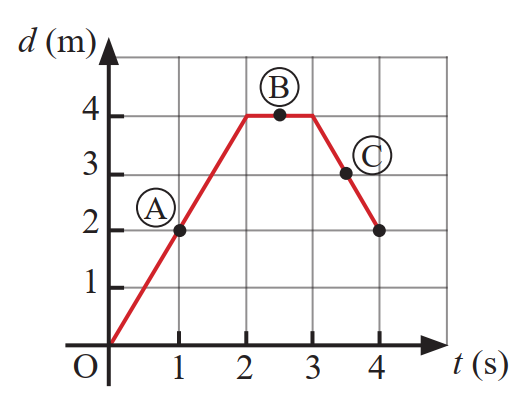
\includegraphics[scale=0.4]{figs/G10Y25B3-21}
		\captionof{figure}{}
		\label{fig:5.3}
	\end{center}
	\loigiai{
		Tốc độ tức thời tại một thời điểm chính là độ dốc của tiếp tuyến với đồ thị ($d$-$t$) tại điểm đó. Trong chuyển động thẳng đều, tốc độ tức thời bằng tốc độ trung bình trên đoạn đó, và bằng giá trị tuyệt đối của hệ số góc của đoạn thẳng trên đồ thị độ dịch chuyển – thời gian.
		\begin{itemize}
			\item Tốc độ tức thời tại $A$ (tại $t=\SI{1}{s}$): Đây là đoạn từ $t=\SI{0}{s}$ đến $t=\SI{1}{s}$.
			$$v_A=\dfrac{\left|d_A - d_0\right|}{t_A - t_0}=\dfrac{\left|2-0\right|}{1-0}=\SI{2}{m/s}.$$
			\item Tốc độ tức thời tại điểm $B$ (tại $t=\SI{3}{s}$): Đây là đoạn từ $t=\SI{2}{s}$ đến $t=\SI{3}{s}$ (hoặc rộng hơn là từ $t=\SI{2}{s}$ đến $t=\SI{4}{s}$).
			$$v_B=\dfrac{\left|d_B - d_{t=2\si{s}}\right|}{t_B - t_{t=2\si{s}}}=\dfrac{\left|4-4\right|}{3-2}=\SI{0}{m/s}.$$
			\item Tốc độ tức thời tại điểm $C$ (tại $t=\SI{4}{s}$): Đây là đoạn từ $t=\SI{3}{s}$ đến $t=\SI{4}{s}$ (hoặc rộng hơn là từ $t=\SI{2}{s}$ đến $t=\SI{4}{s}$).
			$$v_C=\dfrac{\left|d_C - d_{t=3\si{s}}\right|}{t_C - t_{t=3\si{s}}}=\dfrac{\left|2-4\right|}{4-3}=\SI{2}{m/s}.$$
		\end{itemize}
	}
\end{vd}

\begin{vd}
	Đồ thị độ dịch chuyển – thời gian trong chuyển động thẳng của một xe ô tô đồ chơi điều khiển từ xa được vẽ ở hình \ref{fig:5.4}.
	\begin{center}
		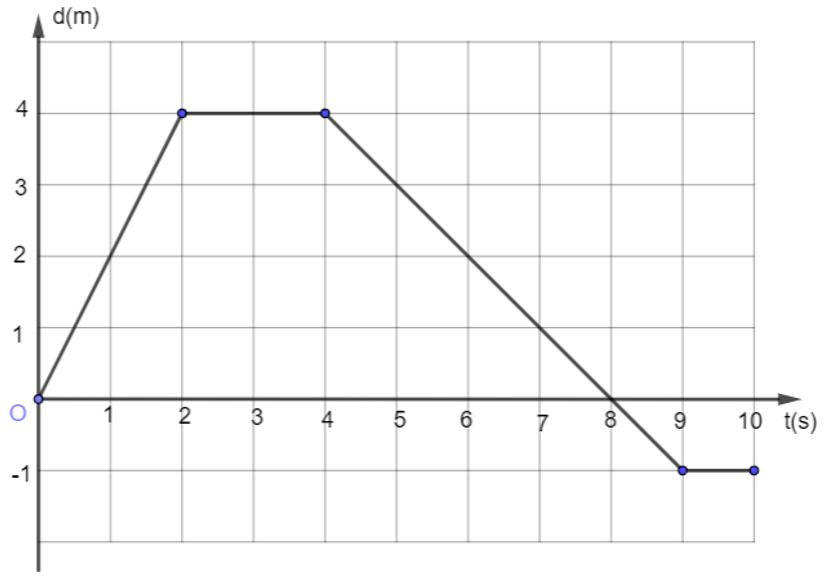
\includegraphics[scale=0.5]{figs/G10Y25B3-20}
		\captionof{figure}{}
		\label{fig:5.4}
	\end{center}
	\begin{enumerate}[label=\alph*)]
		\item Mô tả chuyển động của xe.
		\item Xác định vị trí của xe so với điểm xuất phát của xe ở giây thứ 2, giây thứ 4, giây thứ 8 và giây thứ 10.
		\item Xác định tốc độ và vận tốc của xe trong 2 giây đầu, từ giây 2 đến giây 4 và từ giây 4 đến giây 8.
		\item Xác định quãng đường đi được và độ dịch chuyển của xe sau 10 giây chuyển động. Tại sao giá trị của chúng không giống nhau?
	\end{enumerate}
	\loigiai{
		\begin{enumerate}[label=\alph*)]
			\item **Mô tả chuyển động của xe:**
			\begin{itemize}
				\item **Từ $\SI{0}{s}$ đến $\SI{2}{s}$:** Xe chuyển động thẳng đều theo chiều dương, độ dịch chuyển tăng từ $\SI{0}{m}$ lên $\SI{4}{m}$.
				\item **Từ $\SI{2}{s}$ đến $\SI{4}{s}$:** Xe dừng lại (độ dịch chuyển không đổi, vẫn ở $\SI{4}{m}$).
				\item **Từ $\SI{4}{s}$ đến $\SI{8}{s}$:** Xe chuyển động thẳng đều theo chiều âm (ngược chiều dương), độ dịch chuyển giảm từ $\SI{4}{m}$ về $\SI{0}{m}$ (về vị trí xuất phát).
				\item **Từ $\SI{8}{s}$ đến $\SI{9}{s}$:** Xe tiếp tục chuyển động thẳng đều theo chiều âm, độ dịch chuyển giảm từ $\SI{0}{m}$ xuống $\SI{-1}{m}$.
				\item **Từ $\SI{9}{s}$ đến $\SI{10}{s}$:** Xe dừng lại (độ dịch chuyển không đổi, vẫn ở $\SI{-1}{m}$).
			\end{itemize}
			
			\item **Vị trí của xe so với điểm xuất phát:**
			\begin{itemize}
				\item **Ở giây thứ 2 ($t=\SI{2}{s}$):** Xe cách vị trí xuất phát $\SI{4}{m}$ theo chiều dương ($d=\SI{4}{m}$).
				\item **Ở giây thứ 4 ($t=\SI{4}{s}$):** Xe vẫn cách vị trí xuất phát $\SI{4}{m}$ theo chiều dương ($d=\SI{4}{m}$).
				\item **Ở giây thứ 8 ($t=\SI{8}{s}$):** Xe quay lại vị trí xuất phát ($d=\SI{0}{m}$).
				\item **Ở giây thứ 10 ($t=\SI{10}{s}$):** Xe ở sau vị trí xuất phát $\SI{1}{m}$ ($d=\SI{-1}{m}$).
			\end{itemize}
			
			\item **Tốc độ và vận tốc của xe:**
			\begin{itemize}
				\item **Trong 2 giây đầu (từ $\SI{0}{s}$ đến $\SI{2}{s}$):**
				\begin{itemize}
					\item Độ dịch chuyển: $\Delta d = \SI{4}{m} - \SI{0}{m} = \SI{4}{m}.$
					\item Khoảng thời gian: $\Delta t = \SI{2}{s} - \SI{0}{s} = \SI{2}{s}.$
					\item Vận tốc của xe: $v = \dfrac{\Delta d}{\Delta t} = \dfrac{\SI{4}{m}}{\SI{2}{s}} = \SI{2}{m/s}.$
					\item Tốc độ của xe: $|v| = |\SI{2}{m/s}| = \SI{2}{m/s}.$
				\end{itemize}
				\item **Từ giây 2 đến giây 4 (từ $\SI{2}{s}$ đến $\SI{4}{s}$):**
				\begin{itemize}
					\item Độ dịch chuyển: $\Delta d = \SI{4}{m} - \SI{4}{m} = \SI{0}{m}.$
					\item Khoảng thời gian: $\Delta t = \SI{4}{s} - \SI{2}{s} = \SI{2}{s}.$
					\item Vận tốc của xe: $v = \dfrac{\SI{0}{m}}{\SI{2}{s}} = \SI{0}{m/s}.$
					\item Tốc độ của xe: $|v| = |\SI{0}{m/s}| = \SI{0}{m/s}.$
				\end{itemize}
				\item **Từ giây 4 đến giây 8 (từ $\SI{4}{s}$ đến $\SI{8}{s}$):**
				\begin{itemize}
					\item Độ dịch chuyển: $\Delta d = \SI{0}{m} - \SI{4}{m} = \SI{-4}{m}.$
					\item Khoảng thời gian: $\Delta t = \SI{8}{s} - \SI{4}{s} = \SI{4}{s}.$
					\item Vận tốc của xe: $v = \dfrac{\SI{-4}{m}}{\SI{4}{s}} = \SI{-1}{m/s}.$
					\item Tốc độ của xe: $|v| = |\SI{-1}{m/s}| = \SI{1}{m/s}.$
				\end{itemize}
			\end{itemize}
			
			\item **Quãng đường đi được và độ dịch chuyển sau 10 giây:**
			\begin{itemize}
				\item **Quãng đường đi được ($s$):** Là tổng độ dài đoạn đường xe đã đi được, không xét chiều.
				\begin{itemize}
					\item Từ $\SI{0}{s}$ đến $\SI{2}{s}$: Xe đi được $\SI{4}{m}$.
					\item Từ $\SI{2}{s}$ đến $\SI{4}{s}$: Xe đi được $\SI{0}{m}$.
					\item Từ $\SI{4}{s}$ đến $\SI{8}{s}$: Xe đi được $\SI{4}{m}$ (từ $\SI{4}{m}$ về $\SI{0}{m}$).
					\item Từ $\SI{8}{s}$ đến $\SI{9}{s}$: Xe đi được $\SI{1}{m}$ (từ $\SI{0}{m}$ về $\SI{-1}{m}$).
					\item Từ $\SI{9}{s}$ đến $\SI{10}{s}$: Xe đi được $\SI{0}{m}$.
				\end{itemize}
				Tổng quãng đường xe đi được là $s = \SI{4}{m} + \SI{0}{m} + \SI{4}{m} + \SI{1}{m} + \SI{0}{m} = \SI{9}{m}.$
				
				\item **Độ dịch chuyển ($d$):** Là sự thay đổi vị trí của vật, bằng vị trí cuối trừ vị trí đầu.
				Vị trí ban đầu ($t=\SI{0}{s}$): $d_0 = \SI{0}{m}$.
				Vị trí cuối cùng ($t=\SI{10}{s}$): $d_{10} = \SI{-1}{m}$.
				Độ dịch chuyển sau $\SI{10}{s}$: $d = d_{10} - d_0 = \SI{-1}{m} - \SI{0}{m} = \SI{-1}{m}.$
			\end{itemize}
			
			**Tại sao giá trị của chúng không giống nhau?**
			Giá trị của quãng đường đi được ($\SI{9}{m}$) và độ dịch chuyển ($\SI{-1}{m}$) không giống nhau vì vật đã **đổi chiều chuyển động** trong quá trình di chuyển (từ $\SI{4}{s}$ đến $\SI{9}{s}$ xe chuyển động ngược lại so với ban đầu).
			\begin{itemize}
				\item **Quãng đường đi được** là tổng chiều dài quỹ đạo mà vật đã đi, luôn là một giá trị không âm và chỉ phụ thuộc vào lộ trình.
				\item **Độ dịch chuyển** là một đại lượng vectơ, chỉ phụ thuộc vào vị trí ban đầu và vị trí cuối cùng của vật. Nó có thể dương, âm hoặc bằng 0, và cho biết cả khoảng cách lẫn hướng so với điểm xuất phát.
			\end{itemize}
			Khi vật chuyển động thẳng và không đổi chiều, độ lớn của quãng đường đi được và độ dịch chuyển sẽ bằng nhau. Tuy nhiên, khi vật đổi chiều, tổng quãng đường sẽ lớn hơn độ lớn của độ dịch chuyển.
		\end{enumerate}}
	\end{vd}
\begin{dang}{Xây dựng đồ thị tọa độ - thời gian, chọn tỉ xích, lập bảng giá trị tương ứng cho một vật chuyển động thẳng đều}
\end{dang}
\begin{vd}
	Vật chuyển động thẳng đều có đồ thị tọa độ - thời gian như hình vẽ. Phương trình chuyển động của vật có dạng nào sau đây?
	\begin{center}
		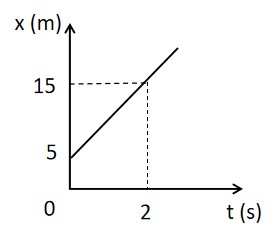
\includegraphics[scale=0.6]{figs/G10Y25B3-22}
	\end{center}
	\choice
	{\True $x=5+5t$.}
	{$x=4t$.}
	{$x=5-5t$.}
	{$x=5+4t$.}
	\loigiai{
		Đồ thị tọa độ - thời gian là một đường thẳng, cho thấy vật chuyển động thẳng đều.
		Từ đồ thị, ta có thể xác định các thông số:
		\begin{itemize}
			\item **Tọa độ ban đầu ($x_0$):** Tại $t = 0$, đồ thị đi qua điểm có tọa độ $x = \SI{5}{m}$. Vậy $x_0 = \SI{5}{m}$.
			\item **Vận tốc ($v$):** Vận tốc của vật được tính bằng độ dốc của đồ thị. Chọn hai điểm rõ ràng trên đồ thị, ví dụ điểm $(\SI{0}{s}, \SI{5}{m})$ và $(\SI{2}{s}, \SI{15}{m})$.
			$$v = \dfrac{\Delta x}{\Delta t} = \dfrac{x_2 - x_1}{t_2 - t_1} = \dfrac{\SI{15}{m} - \SI{5}{m}}{\SI{2}{s} - \SI{0}{s}} = \dfrac{\SI{10}{m}}{\SI{2}{s}} = \SI{5}{m/s}.$$
		\end{itemize}
		
		Phương trình chuyển động thẳng đều có dạng tổng quát là $x = x_0 + vt$.
		Thay các giá trị đã tìm được vào, ta có phương trình chuyển động của vật:
		$$x = 5 + 5t \qquad \left(\si{\meter}, \si{\second}\right).$$
	}
\end{vd}

\begin{vd}
	Hai xe chuyển động đều trên cùng một đường thẳng, cùng chiều. Tốc độ của xe (I) là $\SI{20}{m/s}$, tốc độ của xe (II) là $\SI{10}{m/s}$. Lúc $t=0$, hai xe cách nhau $\SI{200}{m}$. Chọn gốc tọa độ là vị trí của xe (I) lúc $t=0$, chiều dương là chiều chuyển động của hai xe.
	\begin{enumerate}[label=\alph*)]
		\item Viết phương trình chuyển động của mỗi xe.
		\item Vẽ đồ thị chuyển động của hai xe, từ đồ thị hãy xác định thời điểm và nơi gặp nhau của hai xe.
	\end{enumerate}
	\loigiai{
		\begin{enumerate}[label=\alph*)]
			\item **Viết phương trình chuyển động của mỗi xe:**
			Chọn hệ quy chiếu gồm:
			\begin{itemize}
				\item Gốc tọa độ là vị trí của xe (I) lúc $t=0$.
				\item Chiều dương là chiều chuyển động của hai xe.
				\item Mốc thời gian ($t=0$) là lúc hai xe cách nhau $\SI{200}{m}$.
			\end{itemize}
			
			Xác định các thông số cho từng xe:
			\begin{itemize}
				\item **Xe (I):**
				\begin{itemize}
					\item Vị trí ban đầu ($x_{0\text{(I)}}$): Tại gốc tọa độ, nên $x_{0\text{(I)}} = \SI{0}{m}$.
					\item Vận tốc ($v_{\text{(I)}}$): Tốc độ $\SI{20}{m/s}$, chuyển động theo chiều dương, nên $v_{\text{(I)}} = +\SI{20}{m/s}$.
				\end{itemize}
				Phương trình chuyển động của xe (I) là:
				\begin{equation*}
					x_{\text{(I)}}=x_{0\text{(I)}} + v_{\text{(I)}}t = \SI{0}{} + \SI{20}{} \cdot t = 20t\qquad\left(\si{\meter}, \si{\second}\right).
				\end{equation*}
				
				\item **Xe (II):**
				\begin{itemize}
					\item Vị trí ban đầu ($x_{0\text{(II)}}$): Lúc $t=0$, hai xe cách nhau $\SI{200}{m}$ và chuyển động cùng chiều. Do xe (I) ở gốc, xe (II) phải ở vị trí $\SI{200}{m}$ theo chiều dương. Vậy $x_{0\text{(II)}} = \SI{200}{m}$.
					\item Vận tốc ($v_{\text{(II)}}$): Tốc độ $\SI{10}{m/s}$, chuyển động theo chiều dương, nên $v_{\text{(II)}} = +\SI{10}{m/s}$.
				\end{itemize}
				Phương trình chuyển động của xe (II) là:
				\begin{equation*}
					x_{\text{(II)}}=x_{0\text{(II)}} + v_{\text{(II)}}t = \SI{200}{} + \SI{10}{} \cdot t = 200+10t\qquad\left(\si{\meter}, \si{\second}\right).
				\end{equation*}
			\end{itemize}
			
			\item **Vẽ đồ thị chuyển động và xác định thời điểm, nơi gặp nhau:**
			Để vẽ đồ thị, ta lập bảng giá trị tọa độ theo thời gian cho mỗi xe:
			\begin{center}
				\begin{tabular}{|c|c|c|}
					\hline
					$t\ (\si{\second})$ & $x_{\text{(I)}}\ (\si{\meter})$ & $x_{\text{(II)}}\ (\si{\meter})$ \\
					\hline
					0 & 0 & 200 \\
					10 & 200 & 300 \\
					20 & 400 & 400 \\
					30 & 600 & 500 \\
					\hline
				\end{tabular}
			\end{center}
			Đồ thị chuyển động của hai xe là:
			\begin{center}
				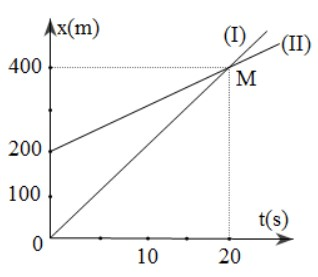
\includegraphics[scale=0.8]{figs/G10Y25B3-23}
			\end{center}
			
			**Xác định thời điểm và nơi gặp nhau từ đồ thị:**
			Hai xe gặp nhau khi tọa độ của chúng bằng nhau, tức là giao điểm của hai đồ thị $x_{\text{(I)}}(t)$ và $x_{\text{(II)}}(t)$.
			Nhìn vào đồ thị, hai đường thẳng cắt nhau tại điểm M có tọa độ $t_M=\SI{20}{s}$ và $x_M=\SI{400}{m}$.
			
			**Kiểm tra bằng phép tính:**
			Hai xe gặp nhau khi $x_{\text{(I)}} = x_{\text{(II)}}$:
			$$20t = 200 + 10t$$
			$$10t = 200$$
			$$t = \dfrac{200}{10} = \SI{20}{s}.$$
			Thay $t = \SI{20}{s}$ vào một trong hai phương trình để tìm vị trí:
			$$x_{\text{(I)}} = 20 \cdot \SI{20}{} = \SI{400}{m}.$$
			
			Vậy, hai xe gặp nhau sau $\SI{20}{s}$ kể từ lúc $t=0$, tại vị trí cách gốc tọa độ (vị trí ban đầu của xe I) một khoảng $\SI{400}{m}$.
		\end{enumerate}	
	}
\end{vd}
\subsection{TRẮC NGHIỆM NHIỀU PHƯƠNG ÁN LỰA CHỌN}
\setcounter{ex}{0}
\Opensolutionfile{ans}[ans/G10Y25B3-TN]
\begin{ex}
	Hãy chọn câu phát biểu đúng?
	\choice
	{Hệ quy chiếu bao gồm hệ toạ độ, mốc thời gian và đồng hồ}
	{Hệ quy chiếu bao gồm vật làm mốc, mốc thời gian và đồng hồ}
	{Hệ quy chiếu bao gồm vật làm mốc, hệ toạ độ, mốc thời gian}
	{\True Hệ quy chiếu bao gồm vật làm mốc, hệ toạ độ, mốc thời gian và đồng hồ}
	\loigiai{
	}
\end{ex}

\begin{ex}
	Kết luận nào sau đây là đúng khi nói về độ dịch chuyển và quãng đường đi được của một vật?
	\choice
	{Độ dịch chuyển và quãng đường đi được đều là đại lượng vô hướng}
	{\True Độ dịch chuyển là đại lượng vectơ còn quãng đường đi được là đại lượng vô hướng}
	{Độ dịch chuyển và quãng đường đi được đều là đại lượng vectơ}
	{Độ dịch chuyển và quãng đường đi được đều là đại lượng không âm}
	\loigiai{
	}
\end{ex}

\begin{ex}
	Một vật bắt đầu chuyển động từ điểm $O$ đến điểm $A$, sau đó chuyển động về điểm $B$. Quãng đường và độ dịch chuyển của vật tương ứng là
	\begin{center}
		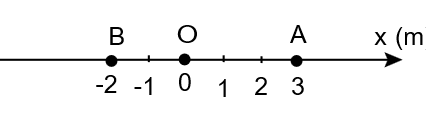
\includegraphics[scale=0.5]{figs/G10Y25B3-7}
	\end{center}
	\choice
	{$\SI{2}{\meter}$; $\SI{-2}{\meter}$}
	{\True $\SI{8}{\meter}$; $\SI{-2}{\meter}$}
	{$\SI{2}{\meter}$; $\SI{2}{\meter}$}
	{$\SI{8}{\meter}$; $\SI{-8}{\meter}$}
	\loigiai{
	}
\end{ex}

\begin{ex}
	Nếu nói “Trái Đất quay quanh Mặt Trời” thì trong câu nói này vật nào được chọn làm mốc
	\choice
	{Cả Mặt Trời và Trái Đất}
	{Trái Đất}
	{Mặt Trăng}
	{\True Mặt Trời}
	\loigiai{
	}
\end{ex}

\begin{ex}
	“Lúc 15 giờ 30 phút hôm qua, xe chúng tôi đang chạy trên quốc lộ 5, cách Hải Dương 10 km”. Việc xác định vị trí của ô tô như trên còn thiếu yếu tố gì?
	\choice
	{Vật làm mốc}
	{\True Chiều dương trên đường đi}
	{Mốc thời gian}
	{Thước đo và đồng hồ}
	\loigiai{
	}
\end{ex}

\begin{ex}
	Trong trường hợp nào dưới đây số chỉ thời điểm mà ta xét trùng với số đo khoảng thời gian trôi?
	\choice
	{Một trận bóng đá diễn ra từ 15 giờ đến 16 giờ 45 phút}
	{Lúc 8 giờ một ô tô khởi hành từ Thành phố Hồ Chí Minh, sau 3 giờ chạy thì xe đến Vũng Tàu}
	{\True Một đoàn tàu xuất phát từ Vinh lúc 0 giờ, đến 8 giờ 05 phút thì đoàn tàu đến Huế}
	{Không có trường hợp nào phù hợp với yêu cầu nêu ra}
	\loigiai{
	}
\end{ex}


\begin{ex}
	Bảng giờ tàu ở bên cho chúng ta biết quãng đường và thời gian mà đoàn tàu SE1 chạy từ ga Huế đến ga Sài Gòn (bỏ qua thời gian tàu đỗ lại các ga) tương ứng là
	\begin{center}
		\begin{tabular}{|c|c|c|}
			\hline
			\thead{Tên ga} & \thead{km} & \thead{SE1}\\
			\hline
			Hà Nội & 0 & 22:15\\
			\hline
			Thanh Hoá & 175& 01:28 (ngày $+1$)\\
			\hline
			Huế & 688 & 11:08 (ngày $+1$)\\
			\hline
			Sài Gòn & 1726 & 06:32 (ngày $+2$)\\
			\hline
		\end{tabular}
	\end{center}
	\choice
	{$\SI{1726}{\kilo\meter}$, 4 giờ 36 phút}
	{$\SI{1726}{\kilo\meter}$, 19 giờ 24 phút}
	{\True $\SI{1038}{\kilo\meter}$, 19 giờ 24 phút}
	{$\SI{1038}{\kilo\meter}$, 4 giờ 36 phút}
	\loigiai{
	}
\end{ex}

\begin{ex}
		\immini{Hai người đi xe đạp từ $A$ đến $C$, người thứ nhất đi theo đường từ $A$ đến $B$, rồi từ $B$ đến $C$; người thứ hai đi thẳng từ $A$ đến $C$. Cả hai đều về đích cùng một lúc.\\
			Hãy chọn kết luận \textbf{sai}.
			\choice
			{Người thứ nhất đi được quãng đường $\SI{8}{\kilo\meter}$}
			{Độ dịch chuyển của người thứ nhất và người thứ hai bằng nhau}
			{\True Độ dịch chuyển và quãng đường đi được của người thứ nhất bằng nhau}
			{Độ dịch chuyển của người thứ nhất là $\SI{5.7}{\kilo\meter}$, hướng $\SI{45}{\degree}$ Đông – Bắc}}{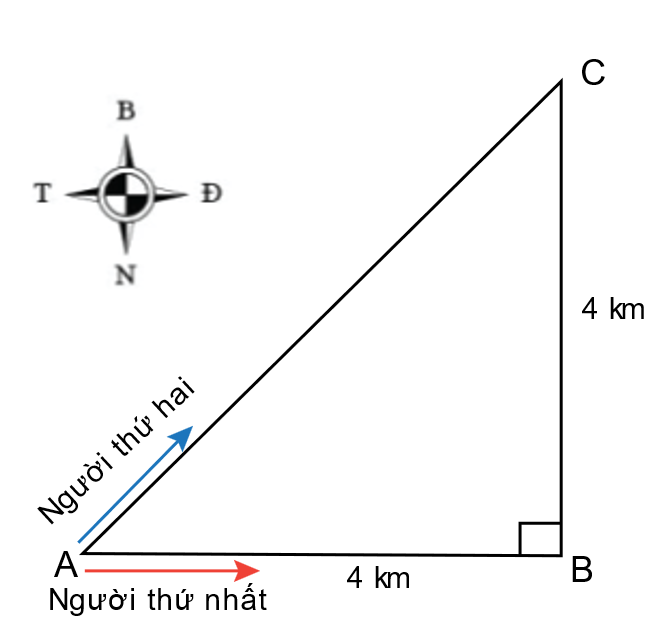
\includegraphics[scale=0.4]{figs/G10Y25B3-6}}
		\loigiai{
		}
\end{ex}

\begin{ex}
	Cho biết Giờ Phối hợp Quốc Tế gọi tắt UTC. So với 0 giờ Quốc Tế, Việt Nam ở múi giờ thứ 7 (UTC+7) và Nhật Bản ở múi giờ thứ 9 (TUC+ 9). Ngày 20/12/2021, máy bay VN300, thuộc hãng hàng không Vietnam Airlines, khởi hành từ Tp. Hồ Chí Minh lúc 0 giờ 20 phút và đến Tp. Tokyo lúc 7 giờ 45 phút, theo giờ địa phương. Thời gian di chuyển của chuyến bay này là
	\choice
	{\True 5 giờ 25 phút}
	{9 giờ 25 phút}
	{7 giờ 25 phút}
	{8 giờ 05 phút}
	\loigiai{
	}
\end{ex}

\begin{ex}
	Chuyến bay từ Thành phố Hồ Chí Minh đi Paris khởi hành lúc 21 giờ 30 phút giờ Hà Nội ngày hôm trước, đến Paris lúc 5 giờ 30 phút sáng hôm sau theo giờ Paris. Biết giờ Paris chậm hơn giờ Hà Nội là 6 giờ. Theo giờ Hà Nội, máy bay đến Paris lúc
	\choice
	{\True 11 giờ 30 phút}
	{14 giờ}
	{12 giờ 30 phút}
	{10 giờ}
	\loigiai{
	}
\end{ex}
\begin{ex}
	Đại lượng đặc trưng cho tính chất nhanh hay chậm của chuyển động là 
	\choice
	{toạ độ}
	{gia tốc}
	{quãng đường đi}
	{\True tốc độ}
	\loigiai{
	}
\end{ex}

\begin{ex}
	Khi nhìn vào tốc kế của ô tô đang chạy, số chỉ trên tốc kế cho ta biết
	\choice
	{gia tốc tức thời của ô tô}
	{vận tốc tức thời của ô tô}
	{\True tốc độ tức thời của ô tô}
	{tốc độ trung bình của ô tô}
	\loigiai{
	}
\end{ex}

\begin{ex}
	Một máy bay phản lực có tốc độ $\SI{700}{\kilo\meter/\hour}$. Nếu muốn bay liên tục trên khoảng cách $\SI{1400}{\kilo\meter}$ thì máy bay phải bay trong thời gian là
	\choice
	{\True $\SI{2}{\hour}$}
	{$\SI{3}{\hour}$}
	{$\SI{2}{\hour}\SI{30}{\minute}$}
	{$\SI{1}{\hour}\SI{30}{\minute}$}
	\loigiai{
		Thời gian máy bay bay quãng đường $\SI{1400}{\kilo\meter}$:
		$$t=\dfrac{s}{v}=\SI{2}{\hour}.$$
	}
\end{ex}

\begin{ex}
	Một xe xuất phát từ lúc 7 giờ 15 phút sáng từ thành phố M, chuyển động thẳng đều tới thành phố N, cách thành phố M $\SI{90}{\kilo\meter}$. Biết tốc độ của xe là $\SI{60}{\kilo\meter/\hour}$, xe đến thành phố N lúc
	\choice
	{9 giờ 45 phút}
	{8 giờ 30 phút}
	{9 giờ 30 phút}
	{\True 8 giờ 45 phút}
	\loigiai{
		Thời gian để xe đi từ M đến N:
		$$\Delta t=\dfrac{s}{v}=\SI{1.5}{\hour}.$$
		Thời điểm xe đến N:
		$$t=\SI{7}{\hour}\SI{15}{\minute}+\Delta t=\SI{8}{\hour}\SI{45}{\minute}.$$
	}
\end{ex}

\begin{ex}
	Một vận động viên chạy cự li $\SI{600}{\meter}$ mất $\SI{74.75}{\second}$. Hỏi vận động viên đó có tốc độ trung bình bao nhiêu?
	\choice
	{\True $\SI{8.03}{\meter/\second}$}
	{$\SI{9.03}{\meter/\second}$}
	{$\SI{10.03}{\meter/\second}$}
	{$\SI{11.03}{\meter/\second}$}
	\loigiai{
		Tốc độ trung bình của vận động viên:
		$$v_\text{tb}=\dfrac{s}{\Delta t}=\SI{8.03}{\meter/\second}.$$
	}
\end{ex}

\begin{ex}
	Trong nội dung thi đấu môn bơi ếch $\SI{100}{\meter}$, một vận động viên đã hoàn thành đường đua với thành tích $\SI{63.25}{\second}$. Tốc độ trung bình của vận động viên này trong giải thi đấu đó là bao nhiêu?
	\choice
	{\True $\SI{1.58}{\meter/\second}$}
	{$\SI{0.63}{\meter/\second}$}
	{$\SI{6.33}{\meter/\second}$}
	{$\SI{36.75}{\meter/\second}$}
	\loigiai{
		Tốc độ trung bình của vận động viên này
		$$v_\text{tb}=\dfrac{s}{t}\approx\SI{1.58}{\meter/\second}.$$
	}
\end{ex}

\begin{ex}
	Một ô tô chạy thử nghiệm trên một đoạn đường thẳng. Cứ $\SI{5}{\second}$ thì có một giọt dầu từ động cơ của ô tô rơi thẳng xuống mặt đường. Hình bên cho thấy mô hình các giọt dầu để lại trên mặt đường. Ô tô chuyển động trên đường này với tốc độ trung bình là
	\begin{center}
		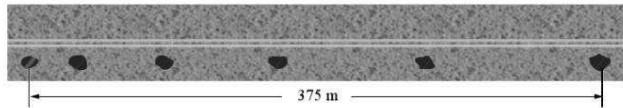
\includegraphics[scale=0.7]{figs/G10Y25B3-15}
	\end{center}
	\choice
	{$\SI{12.5}{\meter/\second}$}
	{\True $\SI{15}{\meter/\second}$}
	{$\SI{30}{\meter/\second}$}
	{$\SI{25}{\meter/\second}$}
	\loigiai{
		Tốc độ trung bình của ô tô:
		$$v_\text{tb}=\dfrac{s}{t}=\dfrac{\SI{375}{\meter}}{\SI{25}{\second}}=\SI{15}{\meter/\second}.$$
	}
\end{ex}

\begin{ex}
	Một chiếc xe ô tô xuất phát từ A lúc 6 giờ sáng, chuyển động thẳng đều tới B, cách A $\SI{120}{\kilo\meter}$. Biết xe tới B lúc 8 giờ 30 phút sáng, tốc độ trung bình của xe là 
	\choice
	{\True $\SI{48}{\kilo\meter/\hour}$}
	{$\SI{45}{\kilo\meter/\hour}$}
	{$\SI{60}{\kilo\meter/\hour}$}
	{$\SI{50}{\kilo\meter/\second}$}
	\loigiai{
		Tốc độ trung bình của xe:
		$$v_\text{tb}=\dfrac{s}{t_2-t_1}=\SI{48}{\kilo\meter/\hour}.$$
	}
\end{ex}

\begin{ex}
	Một xe chuyển động thẳng không đổi chiều, $\SI{1}{\hour}$ đầu xe chạy với tốc độ trung bình $\SI{60}{\kilo\meter/\hour}$ và $\SI{3}{\hour}$ sau xe chạy với tốc độ trung bình $\SI{40}{\kilo\meter/\hour}$. Tính tốc độ trung bình của xe trong suốt thời gian chuyển động.
	\choice
	{$\SI{48}{\kilo\meter/\hour}$}
	{$\SI{40}{\kilo\meter/\hour}$}
	{$\SI{58}{\kilo\meter/\hour}$}
	{\True $\SI{45}{\kilo\meter/\hour}$}
	\loigiai{
		$$v_{tb}=\dfrac{v_1t_1+v_2t_2}{t_1+t_2}=\SI{45}{\kilo\meter/\hour}.$$
	}
\end{ex}

\begin{ex}
	Một người đi xe đạp trên $\dfrac{2}{3}$ đoạn đường đầu với tốc độ trung bình $\SI{10}{\kilo\meter/\hour}$ và $\dfrac{1}{3}$ đoạn đường sau với tốc độ trung bình $\SI{20}{\kilo\meter/\hour}$. Tốc độ trung bình của người đi xe đạp trên cả quãng đường là
	\choice
	{\True $\SI{12}{\kilo\meter/\hour}$}
	{$\SI{15}{\kilo\meter/\hour}$}
	{$\SI{17}{\kilo\meter/\hour}$}
	{$\SI{13.3}{\kilo\meter/\hour}$}
	\loigiai{
		Gọi $s$ là chiều dài đoạn đường
		$$v_{tb}=\dfrac{s}{t_1+t_2}=\dfrac{s}{\dfrac{2s}{3v_1}+\dfrac{s}{3v_2}}=\dfrac{1}{\dfrac{2}{3v_1}+\dfrac{1}{3v_2}}=\SI{12}{\kilo\meter/\hour}.$$
	}
\end{ex}
\begin{ex}
	Khi vật chuyển động thẳng đều cùng chiều dương thì đồ thị $d - t$ của vật có dạng là
	\choice
	{đường thẳng vuông góc với trục $Od$}
	{\True đường thẳng xiên góc đi lên}
	{đường thẳng xiên góc đi xuống}
	{đường thẳng vuông góc với trục $Ot$}
	\loigiai{}
\end{ex}

\begin{ex}
	\immini{Cho đồ thị độ dịch chuyển – thời gian của một vật như hình. Chọn phát biểu đúng.
		\choice
		{Vật đang chuyển động thẳng đều theo chiều dương}
		{Vật đang chuyển động thẳng đều theo chiều âm}
		{\True Vật đang đứng yên}
		{Vật chuyển động thẳng đều theo chiều dương rồi đổi chiều chuyển động ngược lại}}{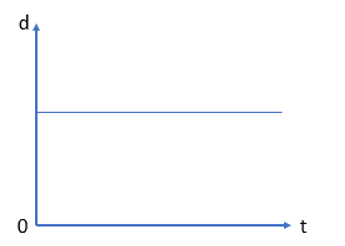
\includegraphics[scale=0.5]{figs/G10Y25B3-24}}
	\loigiai{}
\end{ex}

\begin{ex}
	\immini{Cho đồ thị độ dịch chuyển – thời gian của một vật như hình. Chọn phát biểu đúng.
		\choice
		{Vật đang chuyển động thẳng đều theo chiều dương}
		{Vật đang chuyển động thẳng đều theo chiều âm}
		{Vật đang đứng yên}
		{\True Vật chuyển động thẳng đều theo chiều dương rồi đổi chiều chuyển động ngược lại}}
		{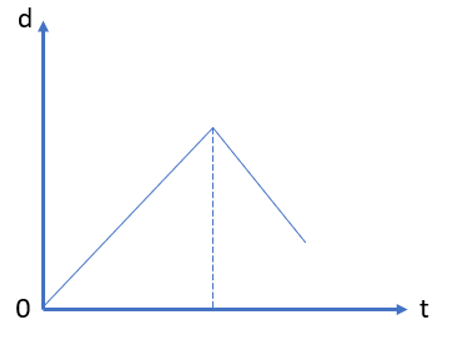
\includegraphics[scale=0.4]{figs/G10Y25B3-25}}
	\loigiai{}
\end{ex}


\begin{ex}
	Đồ thị độ dịch chuyển – thời gian trong chuyển động thẳng của một chất điểm có dạng như hình vẽ.
	\immini{Trong thời gian nào xe chuyển động thẳng đều?
		\choice
		{\True Trong khoảng thời gian từ $0$ đến $t_1$}
		{Trong khoảng thời gian từ $0$ đến $t_2$}
		{Trong khoảng thời gian từ $t_1$ đến $t_2$}
		{Không có lúc nào xe chuyển động thẳng đều}}{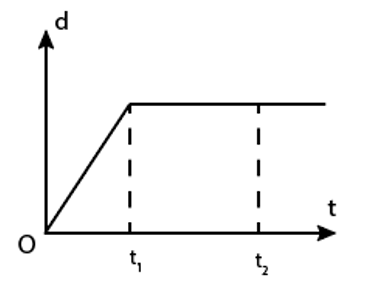
\includegraphics[width=0.5\linewidth]{figs/G10Y25B3-26}}
	\loigiai{}
\end{ex}

\begin{ex}
	{Phương trình chuyển động của một chất điểm dọc theo trục $Ox$ có dạng: $x = 5 + 60t$ ($x$ đo bằng kilomét và $t$ đo bằng giờ). Chất điểm đó xuất phát từ điểm nào và chuyển động với vận tốc bằng bao nhiêu?
		\choice
		{Từ điểm $O$, với vận tốc $\SI{5}{\kilo\meter/\hour}$}
		{Từ điểm $O$, với vận tốc $\SI{60}{\kilo\meter/\hour}$}
		{Từ điểm $M$ cách $O$ $\SI{5}{\kilo\meter}$, với vận tốc $\SI{5}{\kilo\meter/\hour}$}
		{\True Từ điểm $M$ cách $O$ $\SI{5}{\kilo\meter}$, với vận tốc $\SI{60}{\kilo\meter/\hour}$}
	}
	\loigiai{}
\end{ex}

\begin{ex}
	{Phương trình chuyển động của một chất điểm dọc theo $Ox$ có dạng: $x=5t-12$ ($\si{\kilo\meter}$), với $t$ đo bằng giờ. Độ dời của chất điểm từ $\SI{2}{\hour}$ đến $\SI{4}{\hour}$ là
		\choice
		{$\SI{8}{\kilo\meter}$}
		{$\SI{6}{\kilo\meter}$}
		{\True $\SI{10}{\kilo\meter}$}
		{$\SI{2}{\kilo\meter}$}
	}
	\loigiai{}
\end{ex}

\begin{ex}
	{Phương trình chuyển động của một chất điểm dọc theo trục $Ox$ có dạng: $x = 4 -10t$ ($x$ đo bằng kilomét và $t$ đo bằng giờ). Quãng đường đi được của chất điểm sau $\SI{2}{\hour}$ chuyển động là
		\choice
		{$\SI{-20}{\kilo\meter}$}
		{\True $\SI{20}{\kilo\meter}$}
		{$\SI{-8}{\kilo\meter}$}
		{$\SI{8}{\kilo\meter}$}
	}
	\loigiai{}
\end{ex}

\begin{ex}
	\immini{Hình vẽ bên là đồ thị độ dịch chuyển - thời gian của một chiếc xe ô tô chạy từ $A$ đến $B$ trên một đường thẳng. Vận tốc của xe bằng
		\choice
		{\True $\SI{30}{\kilo\meter/\hour}$}
		{$\SI{150}{\kilo\meter/\hour}$}
		{$\SI{120}{\kilo\meter/\hour}$}
		{$\SI{100}{\kilo\meter/\hour}$}}{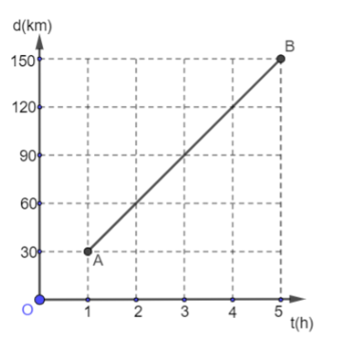
\includegraphics[scale=0.6]{figs/G10Y25B3-27}}
	\loigiai{}
\end{ex}

\begin{ex}\immini{Đồ thị độ dịch chuyển – thời gian của một vật chuyển động như hình vẽ. Vật chuyển động
		\choice
		{\True ngược chiều dương với tốc độ $\SI{20}{\kilo\meter/\hour}$}
		{cùng chiều dương với tốc độ $\SI{20}{\kilo\meter/\hour}$}
		{ngược chiều dương với tốc độ $\SI{60}{\kilo\meter/\hour}$}
		{cùng chiều dương với tốc độ $\SI{60}{\kilo\meter/\hour}$}}{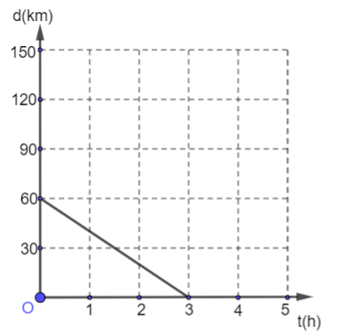
\includegraphics[scale=0.5]{figs/G10Y25B3-28}}

	\loigiai{}
\end{ex}

\begin{ex}
	\immini{Một chất điểm chuyển động trên một đường thẳng. Đồ thị độ dịch chuyển theo thời gian của chất điểm được mô tả như hình vẽ. Tốc độ trung bình của chất điểm trong khoảng thời gian từ 0 đến $\SI{5}{\second}$ là
		\choice
		{$\SI{1.6}{\centi\meter/\second}$}
		{$\SI{6.4}{\centi\meter/\second}$}
		{$\SI{4.8}{\centi\meter/\second}$}
		{\True $\SI{2.4}{\centi\meter/\second}$}}{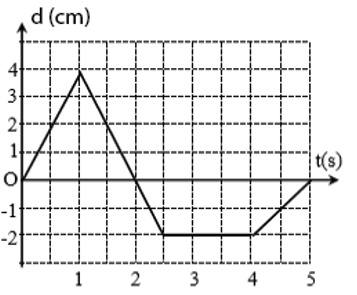
\includegraphics[scale=0.5]{figs/G10Y25B3-29}}
	\loigiai{}
\end{ex}

\begin{ex}
Một người đi bằng thuyền với tốc độ $\SI{2}{m/s}$ về phía đông. Sau khi đi được $\SI{2.2}{\kilo\meter}$, người này lên ô tô đi về phía bắc trong 15 phút với tốc độ $\SI{60}{\kilo\meter/\hour}$. Hãy chọn kết luận \textbf{sai}.
		\choice
		{Tổng quãng đường đã đi là $\SI{17.2}{\kilo\meter}$}
		{Độ dịch chuyển là $\SI{15.2}{\kilo\meter}$}
		{Tốc độ trung bình là $\SI{8.6}{m/s}$}
		{\True Vận tốc trung bình bằng $\SI{8.6}{m/s}$}
	\loigiai{}
\end{ex}

\begin{ex}
Một người bơi dọc theo chiều dài $\SI{100}{m}$ của bể bơi hết $\SI{60}{s}$ rồi quay về lại chỗ xuất phát trong $\SI{70}{s}$. Trong suốt quãng đường đi và về tốc độ trung bình, vận tốc trung bình của người đó lần lượt là
		\choice
		{\True $\SI{1.538}{m/s}$; $\SI{0}{m/s}$}
		{$\SI{1.538}{m/s}$; $\SI{1.876}{m/s}$}
		{$\SI{3.077}{m/s}$; $\SI{2}{m/s}$}
		{$\SI{7.692}{m/s}$; $\SI{2.2}{m/s}$}
	\loigiai{}
\end{ex}

\begin{ex}
Hãy thiết lập phương trình chuyển động của một ô tô chuyển động thẳng đều biết. Ô tô chuyển động theo chiều dương với vận tốc $\SI{10}{m/s}$ và ở thời điểm $\SI{3}{s}$ thì ô tô có tọa độ $\SI{60}{m}$.
		\choice
		{\True $x=30+10t\qquad\left(\si{\meter}, \si{\second}\right)$}
		{$x=20+10t\qquad\left(\si{\meter}, \si{\second}\right)$}
		{$x=10+20t\qquad\left(\si{\meter}, \si{\second}\right)$}
		{$x=40+10t\qquad\left(\si{\meter}, \si{\second}\right)$}
	\loigiai{}
\end{ex}

\begin{ex}
	Hai trạm dừng chân $A$ và $B$ cách nhau $\SI{72}{\kilo\meter}$. Lúc 7h30 sáng, xe ô tô 1 khởi hành từ $A$ chuyển động thẳng đều về $B$ với tốc độ $\SI{36}{\kilo\meter/\hour}$. Nửa giờ sau, xe ô tô 2 chuyển động thẳng đều từ $B$ đến $A$ và gặp ô tô 1 lúc 8 giờ 30 phút. Tìm tốc độ của xe ô tô thứ hai.
		\choice
		{$v_2=\SI{70}{\kilo\meter/\hour}$}
		{\True $v_2=\SI{72}{\kilo\meter/\hour}$}
		{$v_2=\SI{73}{\kilo\meter/\hour}$}
		{$v_2=\SI{74}{\kilo\meter/\hour}$}
	
	\loigiai{}
\end{ex}

\begin{ex}
	Lúc 7 giờ một người đang ở $A$ chuyển động thẳng đều với vận tốc $\SI{10}{m/s}$ đuổi theo người ở $B$ đang chuyển động thẳng đều với vận tốc $\SI{18}{\kilo\meter/\hour}$. Biết $AB =\SI{36}{\kilo\meter}$. Chọn trục tọa độ trùng với quỹ đạo chuyển động, chiều dương là chiều chuyển động, gốc tọa độ tại A, gốc thời gian là lúc $\SI{7}{\hour}$. Thời điểm và vị trí người thứ nhất đuổi kịp người thứ hai là
		\choice
		{lúc $\SI{2}{\hour}$ cách $A$ $\SI{72}{\kilo\meter}$}
		{lúc $\SI{9}{\hour}$ cách $B$ $\SI{36}{\kilo\meter}$}
		{\True lúc $\SI{9}{\hour}$ cách $A$ $\SI{72}{\kilo\meter}$}
		{lúc $\SI{2}{\hour}$ cách $B$ $\SI{36}{\kilo\meter}$}
	\loigiai{}
\end{ex}

\begin{ex}
	Lúc $\SI{10}{\hour}$ có một xe xuất phát từ $A$ đi về $B$ với tốc độ $\SI{50}{\kilo\meter/\hour}$. Lúc 10h30 một xe khác xuất phát từ $B$ đi về $A$ với tốc độ $\SI{80}{\kilo\meter/\hour}$. Cho $AB =\SI{200}{\kilo\meter}$. Lúc $\SI{11}{\hour}$, hai xe cách nhau
		\choice
		{$\SI{100}{\kilo\meter}$}
		{\True $\SI{110}{\kilo\meter}$}
		{$\SI{150}{\kilo\meter}$}
		{$\SI{160}{\kilo\meter}$}
	
	\loigiai{}
\end{ex}

\begin{ex}
	\immini{Hình dưới là đồ thị độ dịch chuyển - thời gian của hai vật chuyển động thẳng cùng hướng. Tỉ lệ vận tốc $\dfrac{v_A}{v_B}$ là
		\choice
		{$\dfrac{3}{1}$}
		{\True $\dfrac{1}{3}$}
		{$\dfrac{\sqrt{3}}{1}$}
		{$\dfrac{1}{\sqrt{3}}$}}{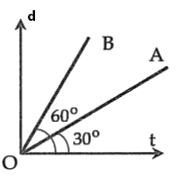
\includegraphics[scale=0.5]{figs/G10Y25B3-30}}
	\loigiai{}
\end{ex}
\Closesolutionfile{ans}
\subsection{TỰ LUẬN VÀ TRẢ LỜI NGẮN}
\setcounter{ex}{0}
\Opensolutionfile{ans}[ans/G10Y25B3-TL]
\begin{ex}
	Khi nào quãng đường và độ di chuyển của một vật có cùng một độ lớn?
	\loigiai{	Chuyển động của vật có quỹ đạo là đường thẳng và không đổi chiều chuyển động.
	}
\end{ex}

\begin{ex}
	Xác định độ dịch chuyển trong các khoảng thời gian liên tiếp bằng nhau của mỗi chuyển động.
	
	\begin{center}
		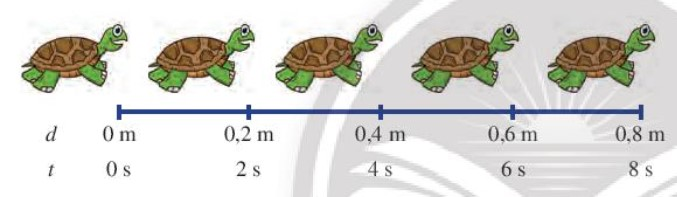
\includegraphics[scale=0.6]{figs/G10Y25B3-8}
	\end{center}
	\loigiai{	
		Độ dịch chuyển trong các khoảng thời gian liên tiếp bằng nhau của mỗi chuyển động
		
		$$\Delta d_1 = x_2 - x_1 = \SI{0,2}{m}.$$
		
		$$\Delta d_2 = x_3 - x_2 = \SI{0,2}{m}.$$
		
		$$\Delta d_3 = x_4 - x_3 = \SI{0,2}{m}.$$
		
		$$\Delta d_4 = x_5 - x_4 = \SI{0,2}{m}.$$
	}
\end{ex}

\begin{ex}
	Hãy xác định các độ dịch chuyển mô tả ở hình trong tọa độ địa lí.
	
	\begin{center}
		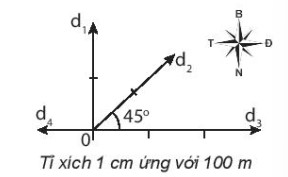
\includegraphics[scale=1]{figs/G10Y25B3-14}
	\end{center}
	\loigiai{	
		Độ dịch chuyển mô tả trên hình là:
		
		$+ d_1 = \SI{200}{m}\ \text{(Bắc)}.$
		
		$+ d_2 = \SI{200}{m}\ \text{(Đông Bắc)}.$
		
		$+ d_3 = \SI{300}{m}\ \text{(Đông)}.$
		
		$+ d_4 = \SI{100}{m}\ \text{(Tây)}.$
	}
\end{ex}

\begin{ex}
	Một ô tô chuyển động trên đường thẳng. Tại thời điểm $t_1$, ô tô ở cách vị trí xuất phát $\SI{5}{km}$. Tại thời điểm $t_2$, ô tô cách vị trí xuất phát $\SI{12}{km}$. Từ $t_1$ đến $t_2$, độ dịch chuyển của ô tô đã thay đổi một đoạn bằng bao nhiêu?
	\loigiai{	
		Từ $t_1$ đến $t_2$, độ dịch chuyển của ô tô thay đổi một đoạn bằng 
		
		$$12-5 = \SI{7}{km}.$$
	}
\end{ex}

\begin{ex}
	Một xe ô tô xuất phát từ tỉnh A, đi đến tỉnh B; rồi lại trở về vị trí xuất phát ở tỉnh A. Xe này đã dịch chuyển, so với vị trí xuất phát một đoạn bằng bao nhiêu? 
	\loigiai{Xe máy này đã dịch chuyển, so với vị trí xuất phát một đoạn là $\SI{0}{km}$.
	}
\end{ex}

\begin{ex}
	Xác định vị trí của vật A trên trục Ox ở hình vẽ tại thời điểm 12h. Biết vật chuyển động thẳng, mỗi giờ đi được $\SI{40}{km}$.
	
	\begin{center}
		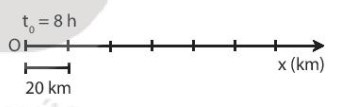
\includegraphics[scale=1]{figs/G10Y25B3-9}
	\end{center}
	\loigiai{	Thời gian vật di chuyển là:
		
		$$12 - 8 = \SI{4}{h}.$$
		
		1 giờ vật di chuyển được $\SI{40}{km}$
		
		$\Rightarrow$ 4 giờ vật di chuyển được: 
		
		$$4 \cdot 40 = \SI{160}{km}.$$
		Tương ứng vật cách gốc toạ độ 8 ô đơn vị.
	}
\end{ex}

\begin{ex}
	Bạn A đi xe đạp từ nhà qua trạm xăng, tới siêu thị mua đồ rồi quay về nhà cất đồ, sau đó đi đến trường. 
	
	\begin{center}
		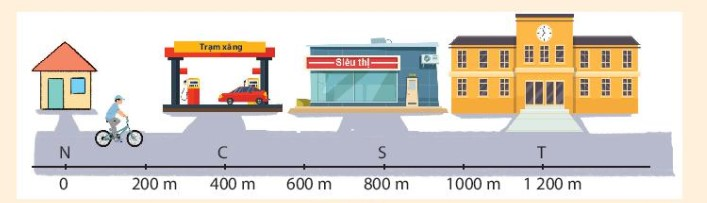
\includegraphics[scale=1]{figs/G10Y25B3-10}
	\end{center}
	Chọn hệ tọa độ có gốc là vị trí nhà bạn A, trục Ox trùng với đường đi từ nhà bạn A đến trường. 
	\begin{enumerate}[label=\alph*)]
		\item Tính quãng đường đi được và độ dịch chuyển của bạn A khi đi từ trạm xăng tới siêu thị.
		\item Tính quãng đường đi được và độ dịch chuyển của bạn A trong cả chuyến đi trên.
	\end{enumerate}
	\loigiai{	
		\begin{enumerate}[label=\alph*)]
			\item Quãng đường bạn A đi từ trạm xăng đến siêu thị là: $$800 - 400 = \SI{400}{m}.$$
			
			Độ dịch chuyển của bạn A từ trạm xăng đến siêu thị là: $$800 - 400 = \SI{400}{m}.$$
			
			\item 
			Quãng đường đi được của bạn A trong cả chuyến đi:
			
			+ Quãng đường bạn A đi từ nhà đến siêu thị là: $\SI{800}{m}.$
			
			+ Quãng đường bạn A quay về nhà cất đồ là: $\SI{800}{m}.$
			
			+ Quãng đường bạn A đi từ nhà đến trường là: $\SI{1200}{m}.$
			
			$\Rightarrow$ Quãng đường đi được của bạn A trong cả chuyến đi là: 	$$ 800 \cdot 2 + 1200 = \SI{2800}{m}.$$ 
			
			Điểm đầu xuất phát của bạn A là nhà, điểm cuối của bạn A là trường.
			
			$\Rightarrow$ Độ dịch chuyển của bạn A là $\SI{1200}{m}.$
			
			Quãng đường đi được và độ dịch chuyển của A trong cả chuyến đi trên là khác nhau. 
		\end{enumerate}
	}
\end{ex}

\begin{ex}
	Hãy so sánh độ lớn của quãng đường đi được và độ dịch chuyển của ba chuyển động. 
	
	\begin{center}
		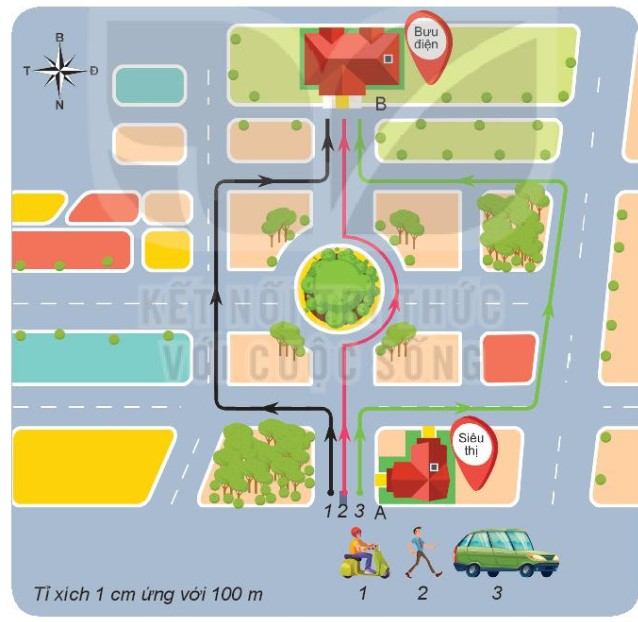
\includegraphics[scale=0.8]{figs/G10Y25B3-11}
	\end{center}
	\loigiai{	
		Quãng đường đi được từ ngắn đến dài: $$2 - 1 - 3.$$
		
		Độ dịch chuyển, ta thấy điểm đầu và điểm cuối của ba chuyển động đều như nhau nên độ dịch chuyển của ba chuyển động bằng nhau.
	}
\end{ex}


\begin{ex}
	Một người lái ô tô đi thẳng $\SI{6}{km}$ theo hướng Tây, sau đó rẽ trái đi thẳng theo hướng Nam $\SI{4}{km}$ rồi quay sang hướng Đông $\SI{3}{km}$. Xác định quãng đường đi được và độ dịch chuyển của ô tô.
	\loigiai{	\begin{center}
			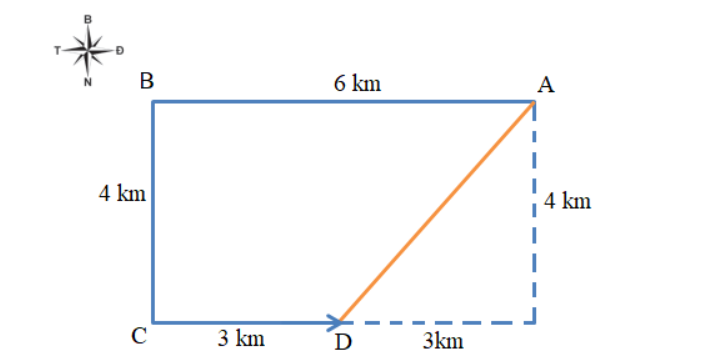
\includegraphics[scale=0.4]{figs/G10Y25B3-12}
		\end{center}
		Quãng đường đi được :
		
		$$s=6+4+3=\SI{13}{km}.$$
		
		Độ dịch chuyển là :
		
		$$d=\sqrt{3^2+4^2}=\SI{5}{\kilo\meter}$$
	}
\end{ex}


\begin{ex}
	Một người bơi ngang từ bờ bên này sang bờ bên kia của một dòng sông rộng $\SI{50}{m}$ có dòng chảy theo hướng từ Bắc xuống Nam. Do nước sông chảy mạnh nên khi sang đến bờ bên kia thì người đó đã trôi xuôi theo dòng nước $\SI{50}{m}$. Xác định độ dịch chuyển của người đó.
	\loigiai{
		\begin{center}
			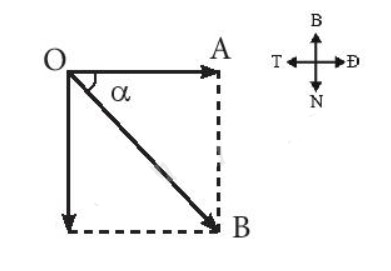
\includegraphics[scale=0.6]{figs/G10Y25B3-13}
		\end{center}
		Người bơi ngang từ bờ bên này sang bên kia theo dự định là OA = $\SI{50}{m}$.
		
		Thực tế, do nước sông chảy mạnh nên vị trí của người đó ở vị trí B, ta có AB = $\SI{50}{m}$.
		
		$\Rightarrow$ Độ dịch chuyển:
		
		$$\Rightarrow\text{OB} = \sqrt{\text{OA}^2 + \text{AB}^2} = \SI{70,7}{m}.$$ 
	}
\end{ex}
\begin{ex}
	Hãy tính tốc độ trung bình ra m/s và km/h của nữ vận động viên tại một số giải thi đấu dựa vào bảng:
	\begin{center}
		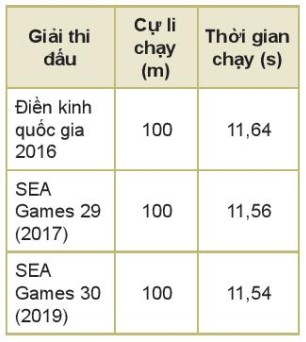
\includegraphics[scale=0.5]{figs/G10Y25B3-16}
	\end{center}
	\loigiai{		Tốc độ trung bình của nữ vận động viên tại giải điền kinh quốc gia 2016 là:
		$$v_\text{tb} = \dfrac{s}{t} =\dfrac{100}{\SI{11.64}{}} = \SI{8.6}{m/s} = \SI{30.96}{\kilo\meter/\hour}.$$
		Tốc độ trung bình của nữ vận động viên tại SEA GAME 19, 2017 là:
		$$v_\text{tb} = \dfrac{s}{t} =\dfrac{100}{\SI{11.56}{}} = \SI{8.65}{m/s} = \SI{31.14}{\kilo\meter/\hour}.$$
		Tốc độ trung bình của nữ vận động viên tại SEA GAME 30, 2019 là:
		$$v_\text{tb} = \dfrac{s}{t} =\dfrac{100}{\SI{11.54}{}}= \SI{8.67}{m/s} = \SI{31.19}{\kilo\meter/\hour}.$$
	}
\end{ex}

\begin{ex}
	Một người đi xe máy đi từ ngã tư với tốc độ trung bình $\SI{30}{\kilo\meter/\hour}$ theo hướng Bắc. Sau 3 phút người đó đến vị trí nào trên hình?
	\begin{center}
		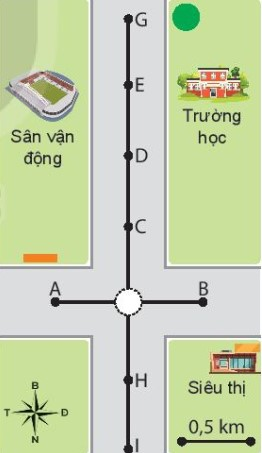
\includegraphics[scale=0.5]{figs/G10Y25B3-17}
	\end{center}
	\loigiai{
		Sau 3 phút người đó đi được quãng đường là:
		
		$$s = vt = \SI{30}{\kilo\meter/\hour} \cdot \SI{3}{\minute} = \SI{30}{\kilo\meter/\hour} \cdot \dfrac{\SI{3}{}}{\SI{60}{}}\ \text{h} = \SI{1.5}{\kilo\meter}.$$
		
		Như vậy người đó đến vị trí điểm E.
	}
\end{ex}

\begin{ex}
	Một ô tô chạy liên tục, trong 2 giờ đầu với tốc độ $\SI{80}{\kilo\meter/\hour}$, trong 1 giờ sau chạy với tốc độ $\SI{50}{\kilo\meter/\hour}$. Tốc độ trung bình của xe trong cả quá trình là bao nhiêu?
	\loigiai{
		Đoạn đường đi được trong 2 giờ đầu:
		$$s_1 = v_1 t_1 = \SI{80}{\kilo\meter/\hour} \cdot \SI{2}{\hour} = \SI{160}{\kilo\meter}.$$
		Đoạn đường đi được trong 1 giờ sau:
		$$s_2 = v_2t_2 = \SI{50}{\kilo\meter/\hour} \cdot \SI{1}{\hour} = \SI{50}{\kilo\meter}.$$
		Tốc độ trung bình của xe:
		$$v_\text{tb} = \dfrac{s_1 + s_2}{t_1 + t_2} = \dfrac{\SI{160}{\kilo\meter} + \SI{50}{\kilo\meter}}{\SI{2}{\hour} + \SI{1}{\hour}} = \dfrac{\SI{210}{\kilo\meter}}{\SI{3}{\hour}} = \SI{70}{\kilo\meter/\hour}.$$
	}
\end{ex}

\begin{ex}
	Một người đi xe bắt đầu cho xe chạy trên đoạn đường thẳng: trong 10 giây đầu xe chạy được quãng đường $\SI{50}{m}$, trong 10 giây tiếp theo xe chạy được $\SI{150}{m}$. Tính tốc độ trung bình của xe máy trong khoảng thời gian nói trên.
	\loigiai{
		Tốc độ trung bình của xe máy:
		$$v_\text{tb} = \dfrac{S_1 + S_2}{t_1 + t_2} = \dfrac{\SI{50}{m} + \SI{150}{m}}{\SI{10}{s} + \SI{10}{s}} = \dfrac{\SI{200}{m}}{\SI{20}{s}} = \SI{10}{m/s}.$$
	}
\end{ex}

\begin{ex}
	Một xe máy điện đi nửa đoạn đường đầu tiên với tốc độ trung bình $v_1 = \SI{24}{\kilo\meter/\hour}$ và nửa đoạn đường sau với tốc độ trung bình $v_2 = \SI{40}{\kilo\meter/\hour}$. Tính tốc độ trung bình trên cả đoạn đường.
	\loigiai{Gọi $2s$ là chiều dài cả đoạn đường.
		
		Thời gian đi nửa đoạn đường đầu:
		$$t_1 = \dfrac{s_1}{v_1} = \dfrac{s}{\SI{24}{\kilo\meter/\hour}}.$$
		Thời gian đi nửa đoạn đường cuối:
		$$t_2 = \dfrac{s_2}{v_2} = \dfrac{s}{\SI{40}{\kilo\meter/\hour}}.$$
		Tốc độ trung bình trên cả đoạn đường của xe máy điện:
		$$v = \dfrac{2s}{t_1 + t_2} = \dfrac{2s}{\dfrac{s}{\SI{24}{\kilo\meter/\hour}} + \dfrac{s}{\SI{40}{\kilo\meter/\hour}}} = \dfrac{2}{\dfrac{1}{\SI{24}{\kilo\meter/\hour}} + \dfrac{1}{\SI{40}{\kilo\meter/\hour}}} = \SI{30}{\kilo\meter/\hour}.$$
	}
\end{ex}

\begin{ex}
	Một ô tô chạy trên đoạn đường thẳng từ A đến B phải mất khoảng thời gian $t$. Trong nửa đầu của khoảng thời gian này ô tô có tốc độ là $\SI{60}{\kilo\meter/\hour}$. Trong nửa khoảng thời gian cuối ô tô có tốc độ là $\SI{40}{\kilo\meter/\hour}$. Tính tốc độ trung bình trên cả đoạn AB.
	\loigiai{
		Quãng đường đi được trong nửa thời gian đầu: $s_1 = v_1 \cdot \dfrac{t}{2} = \SI{60}{\kilo\meter/\hour} \cdot \dfrac{t}{2}.$
		Quãng đường đi được trong nửa thời gian cuối: $s_2 = v_2 \cdot \dfrac{t}{2} = \SI{40}{\kilo\meter/\hour} \cdot \dfrac{t}{2}.$
		Tốc độ trung bình:
		$$v_\text{tb} = \dfrac{S}{t} = \dfrac{s_1 + s_2}{t} = \dfrac{v_1\cdot\dfrac{t}{2}+v_2\cdot\dfrac{t}{2}}{t}=\dfrac{v_1 + v_2}{2} =\dfrac{\SI{60}{\kilo\meter/\hour} + \SI{40}{\kilo\meter/\hour}}{2} = \SI{50}{\kilo\meter/\hour}.$$		
	}
\end{ex}

\begin{ex}
	Một người đi xe đạp từ A đến B với tốc độ $\SI{12}{\kilo\meter/\hour}$ trong $\dfrac{1}{3}$ quãng đường, và tốc độ $\SI{18}{\kilo\meter/\hour}$ trong $\dfrac{2}{3}$ quãng đường còn lại. Tính tốc độ trung bình của người đó trên cả đoạn đường AB.
	\loigiai{
		Gọi $S$ là tổng quãng đường AB.
		Thời gian đi $\dfrac{1}{3}$ quãng đường đầu:
		$$t_1 = \dfrac{S/3}{v_1} = \dfrac{S}{3 \cdot \SI{12}{\kilo\meter/\hour}} = \dfrac{S}{\SI{36}{\kilo\meter/\hour}}.$$
		Thời gian đi $\dfrac{2}{3}$ quãng đường còn lại:
		$$t_2 = \dfrac{2S/3}{v_2} = \dfrac{2S}{3 \cdot \SI{18}{\kilo\meter/\hour}} = \dfrac{2S}{\SI{54}{\kilo\meter/\hour}} = \dfrac{S}{\SI{27}{\kilo\meter/\hour}}.$$
		Tốc độ trung bình của người đó:
		$$v_\text{tb} = \dfrac{S}{t_1 + t_2} = \dfrac{S}{\dfrac{S}{\SI{36}{\kilo\meter/\hour}} + \dfrac{S}{\SI{27}{\kilo\meter/\hour}}} = \dfrac{1}{\dfrac{1}{\SI{36}{\kilo\meter/\hour}} + \dfrac{1}{\SI{27}{\kilo\meter/\hour}}} \approx \SI{15.43}{\kilo\meter/\hour}.$$
	}
\end{ex}

\begin{ex}
	Một chiếc thuyền cao tốc đi từ bến A đến bến B. Trong $\dfrac{2}{3}$ thời gian đầu tốc độ của thuyền là $v_1 = \SI{45}{\kilo\meter/\hour}$, thời gian còn lại thuyền chuyển động với tốc độ $v_2$ bằng bao nhiêu để tốc độ trung bình của nó trên cả quãng đường AB là $v = \SI{48}{\kilo\meter/\hour}$?
	\loigiai{
		Gọi $t$ là tổng thời gian thuyền di chuyển.
		Quãng đường đi được trong $\dfrac{2}{3}$ thời gian đầu: $s_1 = v_1 \cdot \dfrac{2t}{3} = \SI{45}{\kilo\meter/\hour} \cdot \dfrac{2t}{3} = \SI{30}{\kilo\meter/\hour} \cdot t.$
		Quãng đường đi được trong thời gian còn lại ($\dfrac{1}{3}$ thời gian): $s_2 = v_2 \cdot \dfrac{t}{3}.$
		Tốc độ trung bình của thuyền trên đoạn đường AB:
		$$v_\text{tb}=\dfrac{s_1 + s_2}{t} = \dfrac{\SI{30}{\kilo\meter/\hour} \cdot t + v_2 \cdot \dfrac{t}{3}}{t}=\SI{30}{\kilo\meter/\hour}+\dfrac{v_2}{3}.$$
		Theo đề bài, $v_\text{tb} = \SI{48}{\kilo\meter/\hour}$.
		$$\SI{48}{\kilo\meter/\hour} = \SI{30}{\kilo\meter/\hour}+\dfrac{v_2}{3}$$
		$$\Rightarrow \dfrac{v_2}{3} = \SI{48}{\kilo\meter/\hour} - \SI{30}{\kilo\meter/\hour} = \SI{18}{\kilo\meter/\hour}$$
		$$\Rightarrow v_2=\SI{54}{\kilo\meter/\hour}.$$
	}
\end{ex}

\begin{ex}
	Một người đua xe đạp đi trên $\dfrac{1}{3}$ quãng đường đầu với tốc độ $\SI{25}{\kilo\meter/\hour}$. Tính tốc độ của người đó đi trên đoạn đường còn lại. Biết rằng tốc độ trung bình trên cả đoạn đường là $v_\text{tb} = \SI{20}{\kilo\meter/\hour}$.
	\loigiai{
		Gọi $s$ là tổng chiều dài đoạn đường.
		Thời gian đi $\dfrac{1}{3}$ quãng đường đầu: $t_1 = \dfrac{s/3}{v_1} = \dfrac{s}{3 \cdot \SI{25}{\kilo\meter/\hour}} = \dfrac{s}{\SI{75}{\kilo\meter/\hour}}.$
		Thời gian đi $\dfrac{2}{3}$ quãng đường còn lại: $t_2 = \dfrac{2s/3}{v_2} = \dfrac{2s}{3v_2}.$
		Tốc độ trung bình trên cả đoạn đường:
		$$v_\text{tb}=\dfrac{s}{t_1+t_2}=\dfrac{s}{\dfrac{s}{\SI{75}{\kilo\meter/\hour}}+\dfrac{2s}{3v_2}}=\dfrac{1}{\dfrac{1}{\SI{75}{\kilo\meter/\hour}}+\dfrac{2}{3v_2}}$$
		$$ \SI{20}{\kilo\meter/\hour}=\dfrac{1}{\dfrac{1}{\SI{75}{\kilo\meter/\hour}}+\dfrac{2}{3v_2}}$$
		$$\Rightarrow \dfrac{1}{\SI{75}{\kilo\meter/\hour}}+\dfrac{2}{3v_2} = \dfrac{1}{\SI{20}{\kilo\meter/\hour}}$$
		$$\dfrac{2}{3v_2} = \dfrac{1}{\SI{20}{\kilo\meter/\hour}} - \dfrac{1}{\SI{75}{\kilo\meter/\hour}} = \dfrac{15-4}{300}\ \text{h/km} = \dfrac{11}{300}\ \text{h/km}$$
		$$v_2 = \dfrac{2}{3} \cdot \dfrac{300}{11}=\xsi{ \dfrac{200}{11}}{\kilo\meter/\hour}  \approx \SI{18.18}{\kilo\meter/\hour}.$$
	}
\end{ex}

\begin{ex}
	Một ô tô đi trên quãng đường AB với tốc độ trung bình $\SI{54}{\kilo\meter/\hour}$. Nếu giảm tốc độ trung bình đi $\SI{9}{\kilo\meter/\hour}$ thì ôtô đến B trễ hơn dự định 45 phút. Tính quãng đường AB và thời gian dự tính để đi quãng đường đó.
	\loigiai{Gọi $t$ là thời gian dự định để đi quãng đường AB (đơn vị: giờ), $v$ là tốc độ trung bình ban đầu và $s$ là chiều dài quãng đường AB.
		Phương trình chuyển động cho trường hợp đi đúng tốc độ trung bình dự kiến:
		\begin{equation}
			\label{eq:1}
			s=vt=\SI{54}{\kilo\meter/\hour} \cdot t
		\end{equation}
		Khi giảm tốc độ trung bình đi $\SI{9}{\kilo\meter/\hour}$, tốc độ mới là $\SI{54}{\kilo\meter/\hour} - \SI{9}{\kilo\meter/\hour} = \SI{45}{\kilo\meter/\hour}$.
		Thời gian đến B trễ hơn dự định 45 phút, tức là $t + \SI{45}{\minute} = t + \dfrac{\SI{45}{}}{\SI{60}{}}\ \text{h} = t + \SI{0.75}{\hour}$.
		Phương trình chuyển động cho trường hợp đi chậm hơn:
		\begin{equation}
			\label{eq:2}
			s=\left(\SI{54}{\kilo\meter/\hour}- \SI{9}{\kilo\meter/\hour}\right)\left(t+\SI{0.75}{\hour}\right)=\SI{45}{\kilo\meter/\hour}\left(t+\SI{0.75}{\hour}\right)
		\end{equation}
		Từ phương trình (\ref{eq:1}) và phương trình (\ref{eq:2}), ta có:
		$$\SI{54}{\kilo\meter/\hour} \cdot t = \SI{45}{\kilo\meter/\hour}\left(t+\SI{0.75}{\hour}\right)$$
		$$54t = 45t + 45 \cdot 0.75$$
		$$9t = 33.75$$
		$$t = \dfrac{33.75}{9} = \SI{3.75}{\hour}.$$
		Thời gian dự tính để đi quãng đường đó là $\SI{3.75}{\hour}$.
		
		Chiều dài quãng đường AB: $s=\SI{54}{\kilo\meter/\hour} \cdot \SI{3.75}{\hour}=\SI{202.5}{\kilo\meter}$.
	}
\end{ex}

\begin{ex}
	Một cậu bé dắt chó đi dạo về nhà, khi còn cách nhà $\SI{10}{m}$, con chó chạy về nhà với tốc độ $\SI{5}{m/s}$. Vừa đến nhà nó lại chạy ngay lại với tốc độ $\SI{3}{m/s}$. Tính tốc độ trung bình của chú chó trong quãng đường đi được kể từ lúc chạy về nhà đến lúc gặp lại cậu bé, biết cậu bé đi đều với tốc độ $\SI{1}{m/s}$.
	\loigiai{
		Thời gian chú chó chạy từ vị trí cách nhà $\SI{10}{m}$ về đến nhà là:
		$$t_1 = \dfrac{s_1}{v_c} = \dfrac{\SI{10}{m}}{\SI{5}{m/s}} = \SI{2}{s}.$$
		Trong thời gian $t_1$ đó, cậu bé đi được quãng đường là:
		$$s_n = t_1 \cdot v_n = \SI{2}{s} \cdot \SI{1}{m/s} = \SI{2}{m}.$$
		Khoảng cách từ cậu bé đến nhà lúc đó (khi chó đã về đến nhà) là:
		$$s' = \SI{10}{m} - s_n = \SI{10}{m} - \SI{2}{m} = \SI{8}{m}.$$
		Sau đó, chó chạy ngược lại gặp cậu bé. Cậu bé và chó chuyển động ngược chiều về phía nhau.
		Thời gian chú chó chạy từ nhà tới lúc gặp lại cậu bé là:
		$$t_2 = \dfrac{s'}{v_c + v_n} = \dfrac{\SI{8}{m}}{\SI{3}{m/s} + \SI{1}{m/s}} = \dfrac{\SI{8}{m}}{\SI{4}{m/s}} = \SI{2}{s}.$$
		Quãng đường chú chó đã quay lại một đoạn là:
		$$s_2 = v_c \cdot t_2 = \SI{3}{m/s} \cdot \SI{2}{s} = \SI{6}{m}.$$
		Tổng quãng đường chú chó đã đi được kể từ lúc chạy về nhà đến lúc gặp lại cậu bé là:
		$$S_{\text{chó}} = s_1 + s_2 = \SI{10}{m} + \SI{6}{m} = \SI{16}{m}.$$
		Tổng thời gian chú chó chuyển động trong quá trình này là:
		$$T_{\text{chó}} = t_1 + t_2 = \SI{2}{s} + \SI{2}{s} = \SI{4}{s}.$$
		Tốc độ trung bình của chú chó trong quãng đường đi được kể từ lúc chạy về nhà đến lúc gặp lại cậu bé là: 
		$$v_{\text{tb}} = \dfrac{S_{\text{chó}}}{T_{\text{chó}}} = \dfrac{\SI{16}{m}}{\SI{4}{s}} = \SI{4}{m/s}.$$
	}
\end{ex}

\begin{ex}
	Một người đi xe máy chuyển động trên đường thẳng theo 3 giai đoạn: Giai đoạn 1 chuyển động với tốc độ không đổi $v_1 = \SI{30}{\kilo\meter/\hour}$ trong $\SI{10}{\kilo\meter}$ đầu tiên; giai đoạn 2 chuyển động với tốc độ $v_2 = \SI{40}{\kilo\meter/\hour}$ trong 30 phút; giai đoạn 3 chuyển động trên đoạn đường $\SI{4}{\kilo\meter}$ trong 10 phút. Tính tốc độ trung bình trên cả đoạn đường.
	\loigiai{
		Thời gian xe máy chuyển động giai đoạn 1:
		$$t_1 = \dfrac{s_1}{v_1} = \dfrac{\SI{10}{\kilo\meter}}{\SI{30}{\kilo\meter/\hour}} = \dfrac{1}{3}\ \text{h}.$$
		Quãng đường giai đoạn 2:
		$$s_2 = v_2t_2 = \SI{40}{\kilo\meter/\hour} \cdot \SI{30}{\minute} = \SI{40}{\kilo\meter/\hour} \cdot \dfrac{30}{60}\ \text{h} = \SI{20}{\kilo\meter}.$$
		Thời gian giai đoạn 3: $\SI{10}{\minute} = \dfrac{10}{60}\ \text{h} = \dfrac{1}{6}\ \text{h}.$
		
		Tổng quãng đường đã đi:
		$$s = s_1 + s_2 + s_3 = \SI{10}{\kilo\meter} + \SI{20}{\kilo\meter} + \SI{4}{\kilo\meter} = \SI{34}{\kilo\meter}.$$
		Tổng thời gian chuyển động:
		$$t = t_1 + t_2 + t_3 = \dfrac{1}{3}\ \text{h} + \dfrac{30}{60}\ \text{h} + \dfrac{10}{60}\ \text{h} = \dfrac{1}{3}\ \text{h} + \dfrac{1}{2}\ \text{h} + \dfrac{1}{6}\ \text{h} = \dfrac{2+3+1}{6}\ \text{h} = \dfrac{6}{6}\ \text{h} = \SI{1}{\hour}.$$
		Tốc độ trung bình của xe máy trên cả đoạn đường:
		$$v_\text{tb} = \dfrac{s}{t} = \dfrac{\SI{34}{\kilo\meter}}{\SI{1}{\hour}} = \SI{34}{\kilo\meter/\hour}.$$
	}
\end{ex}

\begin{ex}
	Một ô tô chuyển động trên đoạn đường MN. Trong một phần hai quãng đường đầu đi với $v = \SI{40}{\kilo\meter/\hour}$. Trong một phần hai quãng đường còn lại đi trong một phần hai thời gian đầu với $v = \SI{75}{\kilo\meter/\hour}$ và trong một phần hai thời gian cuối đi với $v = \SI{45}{\kilo\meter/\hour}$. Tính tốc độ trung bình trên đoạn MN.
	\loigiai{
		Gọi $S$ là chiều dài đoạn đường MN.
		Nửa quãng đường đầu ($S/2$) đi với tốc độ $v_1 = \SI{40}{\kilo\meter/\hour}$.
		Thời gian đi nửa quãng đường đầu là: $t_1 = \dfrac{S/2}{v_1} = \dfrac{S}{2 \cdot \SI{40}{\kilo\meter/\hour}} = \dfrac{S}{\SI{80}{\kilo\meter/\hour}}.$
		
		Xét nửa quãng đường còn lại ($S/2$). Gọi $t'$ là tổng thời gian đi nửa quãng đường này.
		Trong nửa thời gian đầu ($t'/2$), tốc độ là $v_2 = \SI{75}{\kilo\meter/\hour}$. Quãng đường: $s_{2a} = v_2 \cdot \dfrac{t'}{2}.$
		Trong nửa thời gian cuối ($t'/2$), tốc độ là $v_3 = \SI{45}{\kilo\meter/\hour}$. Quãng đường: $s_{2b} = v_3 \cdot \dfrac{t'}{2}.$
		Tổng quãng đường trong giai đoạn này là $S/2 = s_{2a} + s_{2b} = v_2 \cdot \dfrac{t'}{2} + v_3 \cdot \dfrac{t'}{2} = \dfrac{t'}{2}(v_2 + v_3).$
		Tốc độ trung bình trong nửa quãng đường cuối (từ đây ta có thể tính tốc độ trung bình cho nửa sau):
		$$v_{\text{tb2}}=\dfrac{s_{2a}+s_{2b}}{t'} = \dfrac{\dfrac{t'}{2}(v_2+v_3)}{t'} = \dfrac{v_2+v_3}{2} = \dfrac{\SI{75}{\kilo\meter/\hour}+\SI{45}{\kilo\meter/\hour}}{2} = \dfrac{\SI{120}{\kilo\meter/\hour}}{2} = \SI{60}{\kilo\meter/\hour}.$$
		Thời gian đi nửa quãng đường cuối là: $t_2 = \dfrac{S/2}{v_{\text{tb2}}} = \dfrac{S/2}{\SI{60}{\kilo\meter/\hour}} = \dfrac{S}{\SI{120}{\kilo\meter/\hour}}.$
		
		Tổng thời gian đi trên cả đoạn MN là: $T = t_1 + t_2 = \dfrac{S}{\SI{80}{\kilo\meter/\hour}} + \dfrac{S}{\SI{120}{\kilo\meter/\hour}} = S \left( \dfrac{1}{80} + \dfrac{1}{120} \right)\ \text{h/km} = S \left( \dfrac{3+2}{240} \right)\ \text{h/km} = S \cdot \dfrac{5}{240}\ \text{h/km} = \dfrac{S}{\SI{48}{\kilo\meter/\hour}}.$
		Tốc độ trung bình trên cả đoạn MN:
		$$v_\text{tb}=\dfrac{S}{T} = \dfrac{S}{S/\SI{48}{\kilo\meter/\hour}} = \SI{48}{\kilo\meter/\hour}.$$
	}
\end{ex}

\begin{ex}
	Một người đi xe máy trên một đoạn đường thẳng AB. Trên một phần ba đoạn đường đầu đi với $v_1 = \SI{30}{\kilo\meter/\hour}$, một phần ba đoạn đường tiếp theo với $v_2 = \SI{36}{\kilo\meter/\hour}$ và một phần ba đoạn đường cuối cùng đi với $v_3= \SI{48}{\kilo\meter/\hour}$. Tính $v_\text{tb}$ trên cả đoạn AB.
	\loigiai{
		Gọi $S$ là tổng chiều dài đoạn đường AB.
		Thời gian đi một phần ba đoạn đường đầu: $t_1 = \dfrac{S/3}{v_1} = \dfrac{S}{3 \cdot \SI{30}{\kilo\meter/\hour}} = \dfrac{S}{\SI{90}{\kilo\meter/\hour}}.$
		Thời gian đi một phần ba đoạn đường tiếp theo: $t_2 = \dfrac{S/3}{v_2} = \dfrac{S}{3 \cdot \SI{36}{\kilo\meter/\hour}} = \dfrac{S}{\SI{108}{\kilo\meter/\hour}}.$
		Thời gian đi một phần ba đoạn đường cuối cùng: $t_3 = \dfrac{S/3}{v_3} = \dfrac{S}{3 \cdot \SI{48}{\kilo\meter/\hour}} = \dfrac{S}{\SI{144}{\kilo\meter/\hour}}.$
		
		Tổng thời gian đi trên cả đoạn đường AB là:
		$$T = t_1 + t_2 + t_3 = S \left( \dfrac{1}{90} + \dfrac{1}{108} + \dfrac{1}{144} \right)\ \text{h/km}.$$
		Tìm bội chung nhỏ nhất của 90, 108, 144.
		$90 = 2 \cdot 3^2 \cdot 5$
		$108 = 2^2 \cdot 3^3$
		$144 = 2^4 \cdot 3^2$
		BCNN($90, 108, 144$) = $2^4 \cdot 3^3 \cdot 5 = 16 \cdot 27 \cdot 5 = 2160.$
		
		$$T = S \left( \dfrac{2160/90}{2160} + \dfrac{2160/108}{2160} + \dfrac{2160/144}{2160} \right)\ \text{h/km} = S \left( \dfrac{24+20+15}{2160} \right)\ \text{h/km} = S \cdot \dfrac{59}{2160}\ \text{h/km}.$$
		Tốc độ trung bình trên cả đoạn đường AB:
		$$v_\text{tb}=\dfrac{S}{T} = \dfrac{S}{S \cdot \dfrac{59}{2160}\ \text{h/km}} = \xsi{\dfrac{2160}{59}}{\kilo\meter/\hour}\approx \SI{36.61}{\kilo\meter/\hour}.$$
	}
\end{ex}
\begin{ex}
	Hãy tính quãng đường đi được, độ dịch chuyển, tốc độ, vận tốc của bạn A khi đi từ nhà đến trường và khi đi từ trường đến siêu thị. Coi chuyển động của bạn A là chuyển động đều và biết cứ $\SI{100}{m}$ bạn A đi hết $\SI{25}{s}$.
	\begin{center}
		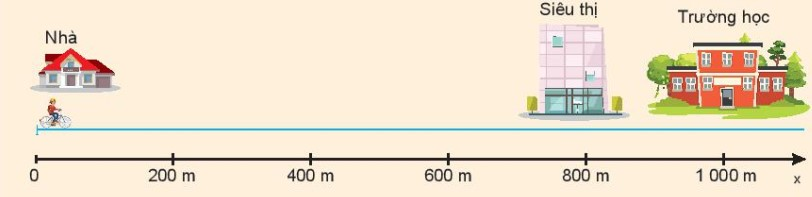
\includegraphics[scale=0.9]{figs/G10Y25B3-31}
	\end{center}
	\loigiai{
		Vì bạn A đi từ nhà đến trường là theo 1 hướng, không đổi hướng nên:
		Quãng đường đi được và độ dịch chuyển là như nhau và bằng $\SI{1000}{m}$.
		Vận tốc và tốc độ là như nhau và bằng:
		$$v = \dfrac{d}{t} = \dfrac{\SI{100}{m}}{\SI{25}{s}} = \SI{4}{m/s}.$$
		Tương tự, khi đi từ trường đến siêu thị thì quãng đường và độ dịch chuyển bằng nhau và bằng $\SI{200}{\meter}$.
	}
\end{ex}

\begin{ex}
	Bạn A đi học từ nhà đến trường theo lộ trình ABC. Biết bạn A đi đoạn đường $\text{AB} = \SI{400}{m}$ hết 6 phút, đoạn đường $\text{BC} = \SI{300}{m}$ hết 4 phút. Xác định tốc độ trung bình và vận tốc trung bình của bạn A khi đi từ nhà đến trường.
	\begin{center}
		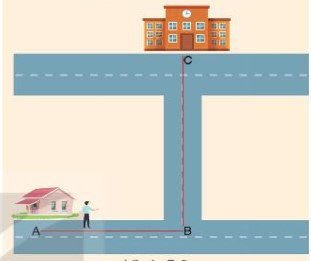
\includegraphics[scale=1]{figs/G10Y25B3-32}
	\end{center}
	\loigiai{
		Độ dịch chuyển của bạn A đến trường chính là độ dài $\text{AC}$.
		Vì AB vuông góc với BC, áp dụng định lý Pitago:
		$$\text{AC} = \sqrt{(\text{AB})^2 + (\text{BC})^2} = \sqrt{(\SI{400}{m})^2 + (\SI{300}{m})^2} = \sqrt{160000 + 90000}\ \si{m} = \sqrt{250000}\ \si{m} = \SI{500}{m}.$$
		Tổng quãng đường bạn A đã đi:
		$$s = \text{AB} + \text{BC} = \SI{400}{m} + \SI{300}{m} = \SI{700}{m}.$$
		Tổng thời gian chuyển động:
		$$t = \SI{6}{phút} + \SI{4}{phút} = \SI{10}{phút} = \SI{10}{} \cdot \SI{60}{s} = \SI{600}{s}.$$
		Tốc độ trung bình:
		$$v_{\text{tốc độ}} = \dfrac{s}{t} = \dfrac{\SI{700}{m}}{\SI{600}{s}} \approx \SI{1.17}{m/s}.$$
		Vận tốc trung bình:
		$$v_{\text{vận tốc}} = \dfrac{\text{AC}}{t} = \dfrac{\SI{500}{m}}{\SI{600}{s}} \approx \SI{0.83}{m/s}.$$
	}
\end{ex}

\begin{ex}
	Hãy vẽ đồ thị độ dịch chuyển - thời gian trong chuyển động của A theo bảng ghi số liệu vào vở. Trên trục tung (trục độ dịch chuyển) $\SI{1}{cm}$ ứng với $\SI{200}{m}$; trên trục hoành (trục thời gian) $\SI{1}{cm}$ ứng với $\SI{50}{s}$.
	\begin{center}
		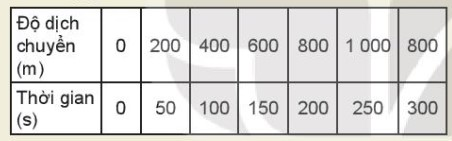
\includegraphics[scale=1]{figs/G10Y25B3-33}
	\end{center}
	\loigiai{
		Từ bảng số liệu ta vẽ được đồ thị như hình sau:
		\begin{center}
			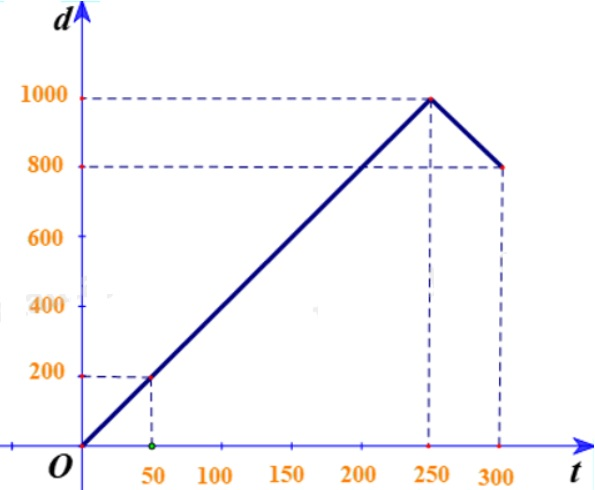
\includegraphics[scale=0.6]{figs/G10Y25B3-34}
		\end{center}
	}
\end{ex}

\begin{ex}
	Đồ thị độ dịch chuyển - thời gian của một người đang bơi trong một bể bơi dài $\SI{50}{m}$.
	\begin{center}
		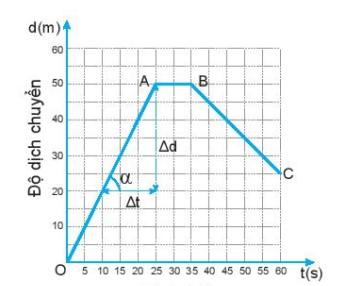
\includegraphics[scale=1]{figs/G10Y25B3-35}
	\end{center}
	\begin{enumerate}[label=\alph*)]
		\item Trong 25 giây đầu mỗi giây người đó bơi được bao nhiêu mét? Tính vận tốc của người đó ra m/s. Từ giây nào đến giây nào người đó không bơi?
		\item Từ giây 35 đến giây 60 người đó bơi theo chiều nào? Trong 20 giây cuối cùng, mỗi giây người đó bơi được bao nhiêu mét? Tính vận tốc của người đó ra m/s.
		\item Xác định độ dịch chuyển và vận tốc của người đó trong cả quá trình bơi.
	\end{enumerate}
	\loigiai{
		\begin{enumerate}[label=\alph*)]
			\item Từ đồ thị, trong 25 giây đầu (từ $\SI{0}{s}$ đến $\SI{25}{s}$), người đó chuyển động thẳng từ vị trí $\SI{0}{m}$ đến $\SI{50}{m}$. Độ dịch chuyển trong 25 giây đầu là $\SI{50}{m}$.
			Mỗi giây người đó bơi được:
			$$\dfrac{\SI{50}{m}}{\SI{25}{s}} = \SI{2}{m/s}.$$
			Vận tốc của người đó trong 25 giây đầu:
			$$v = \dfrac{\Delta d}{\Delta t} = \dfrac{\SI{50}{m} - \SI{0}{m}}{\SI{25}{s} - \SI{0}{s}} = \SI{2}{m/s}.$$
			Từ đồ thị, đoạn từ A đến B (từ giây 25 đến giây 35), độ dịch chuyển không đổi ($\SI{50}{m}$), nghĩa là người đó không bơi. Vậy, người đó không bơi từ giây 25 đến giây 35.
			\item Từ giây 35 đến giây 60, đồ thị đi xuống, nghĩa là độ dịch chuyển giảm. Điều này cho thấy người đó bơi theo chiều ngược lại (ngược chiều dương).
			Trong 20 giây cuối cùng (từ giây 40 đến giây 60):
			\begin{itemize}
				\item Tại $t=\SI{40}{s}$, $d_1 = \SI{45}{m}$.
				\item Tại $t=\SI{60}{s}$, $d_2 = \SI{25}{m}$.
			\end{itemize}
			Trong 20 giây cuối, độ dịch chuyển thay đổi là $\Delta d = d_2 - d_1 = \SI{25}{m} - \SI{45}{m} = \SI{-20}{m}.$
			Quãng đường đi được trong 20 giây cuối: $s = |\Delta d| = |\SI{-20}{m}| = \SI{20}{m}.$
			Mỗi giây người đó bơi được (tốc độ):
			$$\dfrac{\SI{20}{m}}{\SI{20}{s}} = \SI{1}{m/s}.$$
			Vận tốc của người đó trong 20 giây cuối là:
			$$v = \dfrac{\Delta d}{\Delta t} = \dfrac{\SI{25}{m} - \SI{45}{m}}{\SI{60}{s} - \SI{40}{s}} = \dfrac{\SI{-20}{m}}{\SI{20}{s}} = \SI{-1}{m/s}.$$
			\item Trong cả quá trình bơi (từ $\SI{0}{s}$ đến $\SI{60}{s}$):
			\begin{itemize}
				\item Vị trí ban đầu: $d_{\text{bđ}} = \SI{0}{m}$.
				\item Vị trí cuối cùng: $d_{\text{cuối}} = \SI{25}{m}$.
			\end{itemize}
			Độ dịch chuyển của người đó trong cả quá trình bơi:
			$$\Delta d = d_{\text{cuối}} - d_{\text{bđ}} = \SI{25}{m} - \SI{0}{m} = \SI{25}{m}.$$
			Tổng thời gian bơi: $t = \SI{60}{s}$.
			Vận tốc trung bình của người đó trong cả quá trình bơi:
			$$v_{\text{tb}} = \dfrac{\Delta d}{t} = \dfrac{\SI{25}{m}}{\SI{60}{s}} \approx \SI{0.417}{m/s}.$$
		\end{enumerate}
	}
\end{ex}

\Closesolutionfile{ans}